\documentclass[11pt]{article}

% ---------- Packages ----------
\usepackage[margin=1in]{geometry}
\usepackage{amsmath, amssymb}
\usepackage{graphicx}
\usepackage{fancyhdr}
\usepackage{float}
\usepackage{listings}
\usepackage{xcolor}

\lstset{
    language=Matlab,
    basicstyle=\ttfamily\small,
    breaklines=true,
    breakatwhitespace=false,
    columns=fullflexible,
    showstringspaces=false,
    tabsize=4
}

% ---------- Paragraph Formatting ----------
\setlength{\parindent}{0pt}
\setlength{\parskip}{0.5em}

% ---------- Header ----------
\pagestyle{fancy}
\fancyhf{}
\lhead{ASEN 5090 Introduction    GNSS}
\rhead{Justin Le, Elsa Carreras}
\cfoot{\thepage}

% ---------- Document ----------
\begin{document}

% ---------- Title ----------
\begin{center}
    {\Large \textbf{Homework 4}}\\[0.5em]
    {\large ASEN 5090 Introduction to GNSS}\\[0.5em]
    Justin Le, Elsa Carreras\\
    \today
\end{center}

\vspace{1em}

\section*{Problem 1: Starting Point}
\begin{figure}[H]
    \centering
    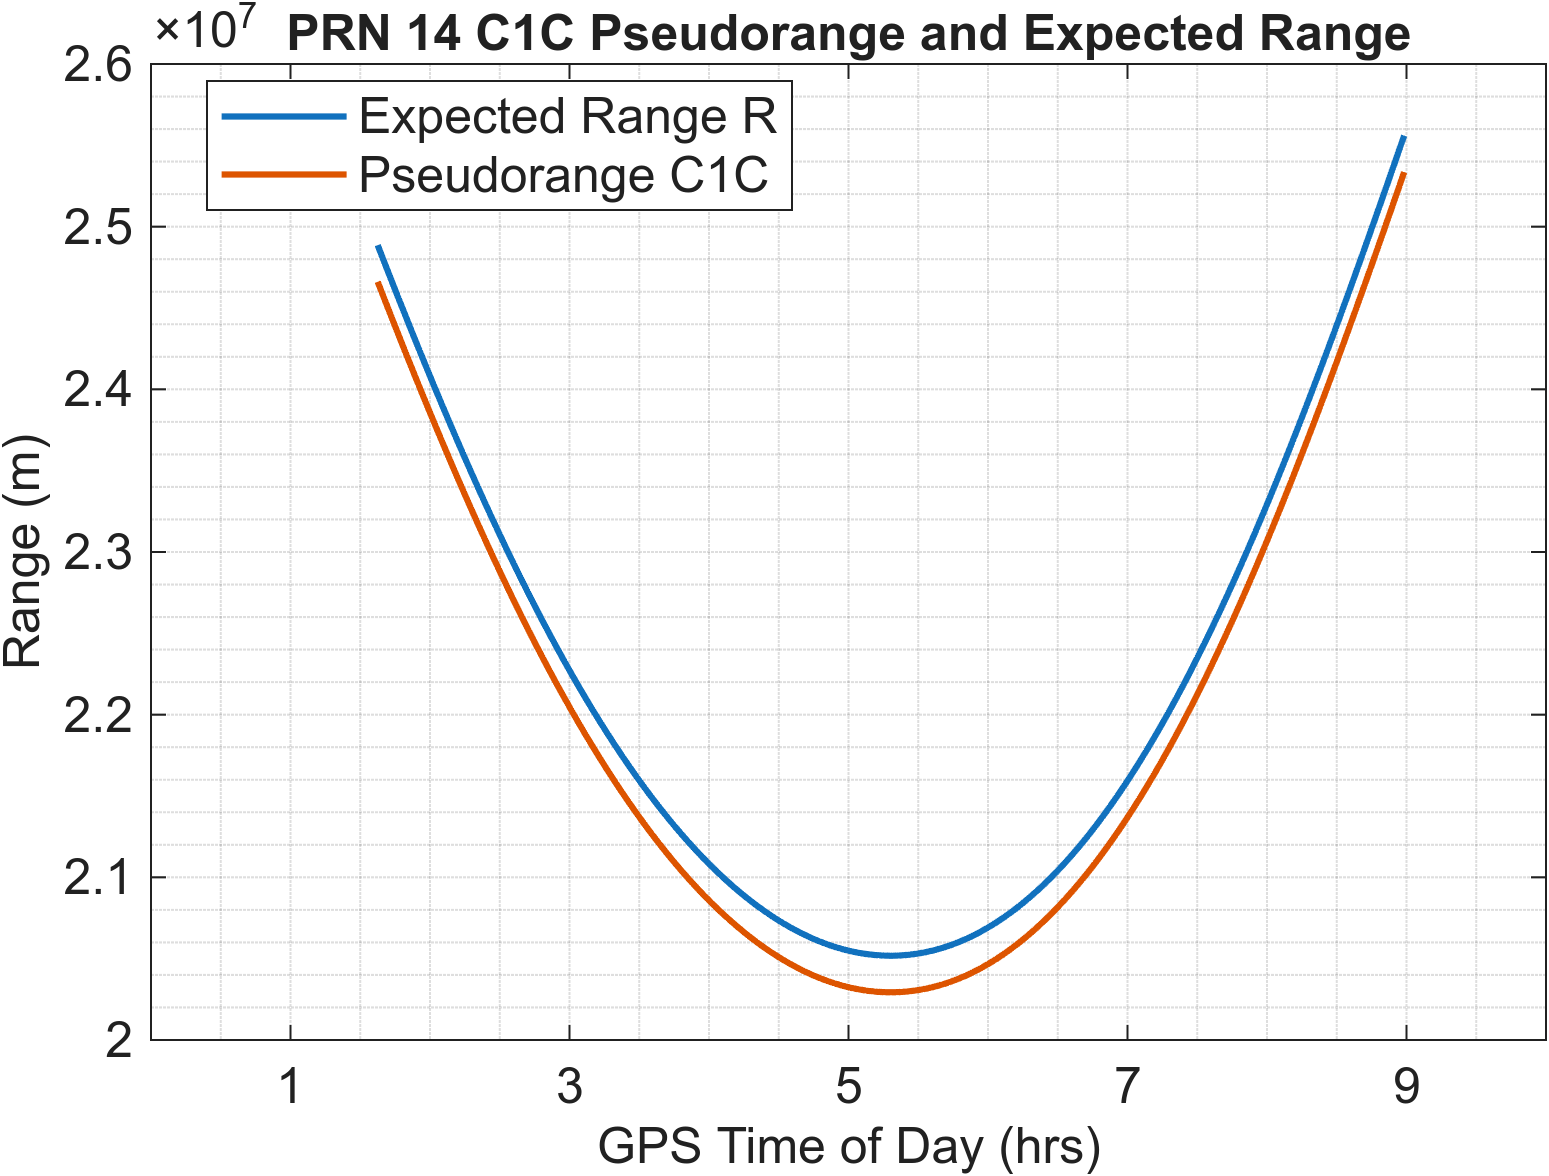
\includegraphics[width=0.6\textwidth]{../MATLAB/figures/HW4/HW4_P1_C1C_vs_R_PRN14.png}
    \caption{Expected Range and C1C Pseudorange}
    \label{fig:Expected Range and C1C Pseudorange}
\end{figure}

\begin{figure}[H]
    \centering
    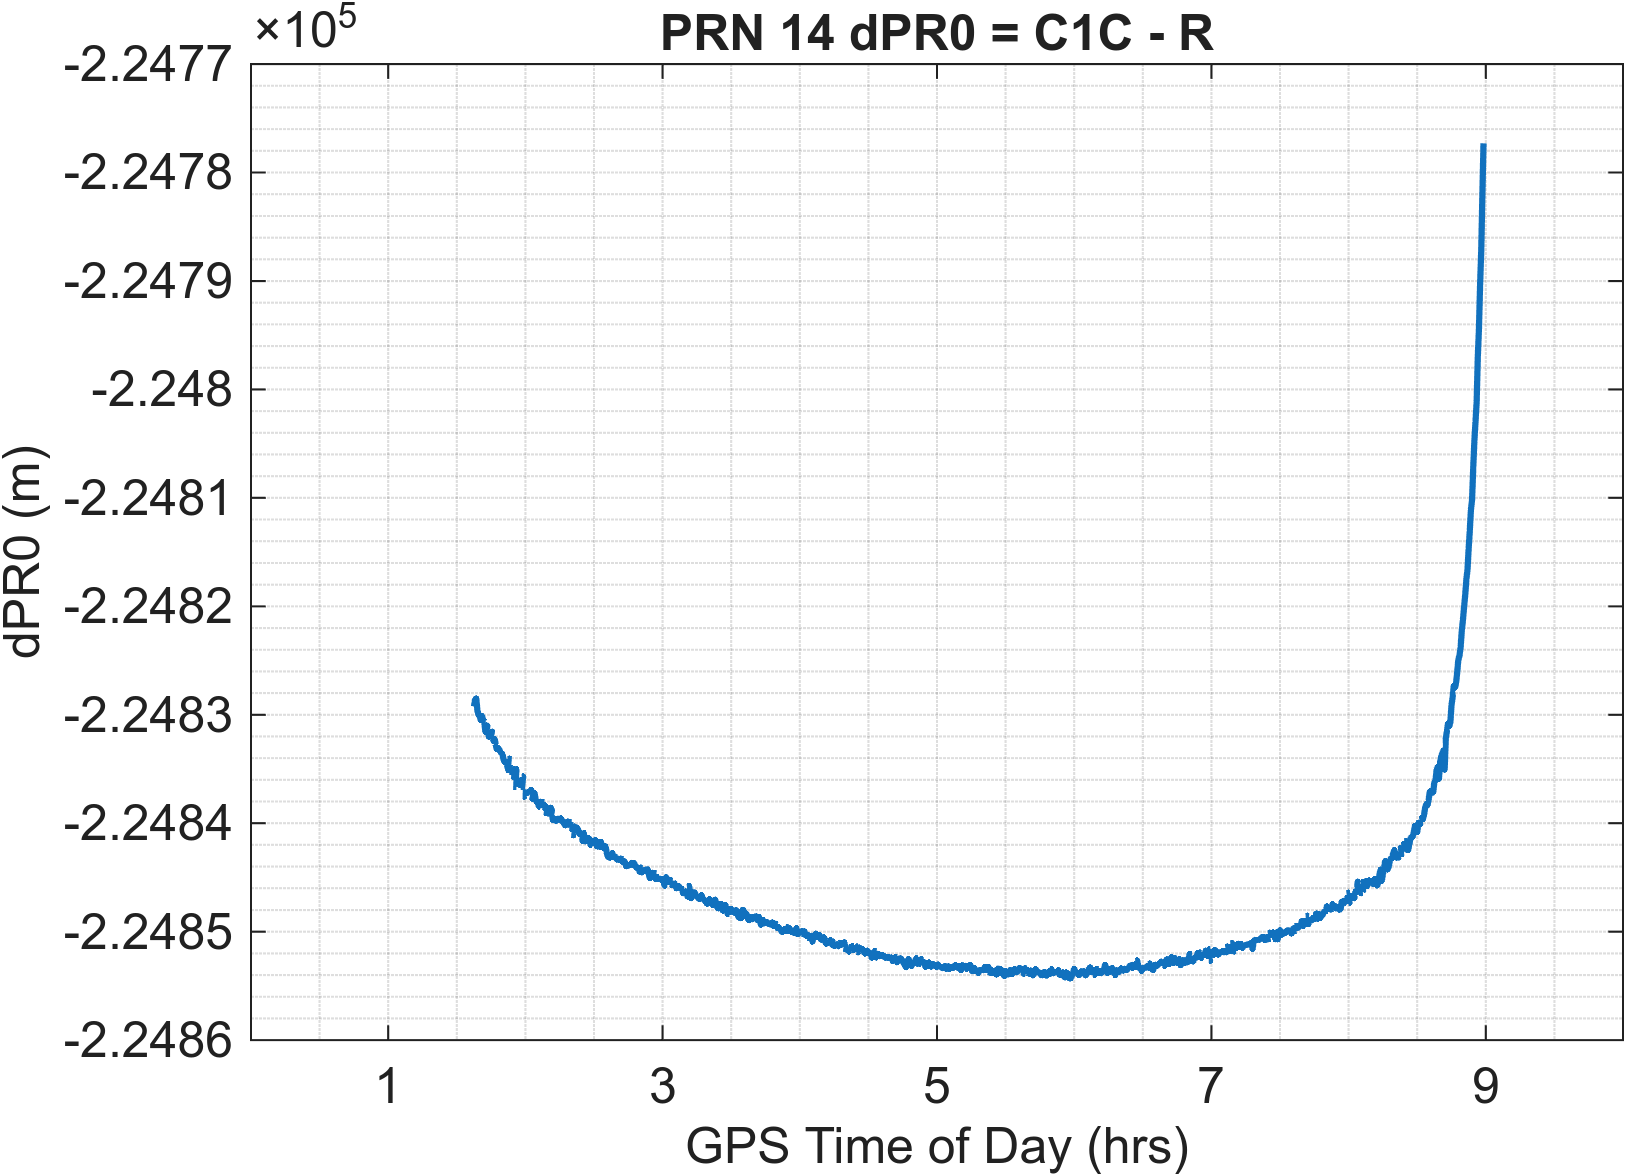
\includegraphics[width=0.6\textwidth]{../MATLAB/figures/HW4/HW4_P1_dPR0_PRN14.png}
    \caption{dPR0 Results}
    \label{fig:dPR0 Results}
\end{figure}

\begin{lstlisting}[language=Matlab]
dPR0 first value: -224829.2307 m
dPR0 last value:  -224777.3128 m
\end{lstlisting}

\hspace*{2em}The results should look very similar to what was plotted for Homework 3 which is noticeable in Figure \ref{fig:dPR0 Results}. We assume we would get residuals of 100s of kilometers since expected range is calculated with orbital parameters and C1C is a signal sent that needs corrections in processing, a large part of this error is from the raw pseudoranges not accounting for clock bias.
\newpage
\section*{Problem 2: Clock Error}
\begin{figure}[H]
    \centering
    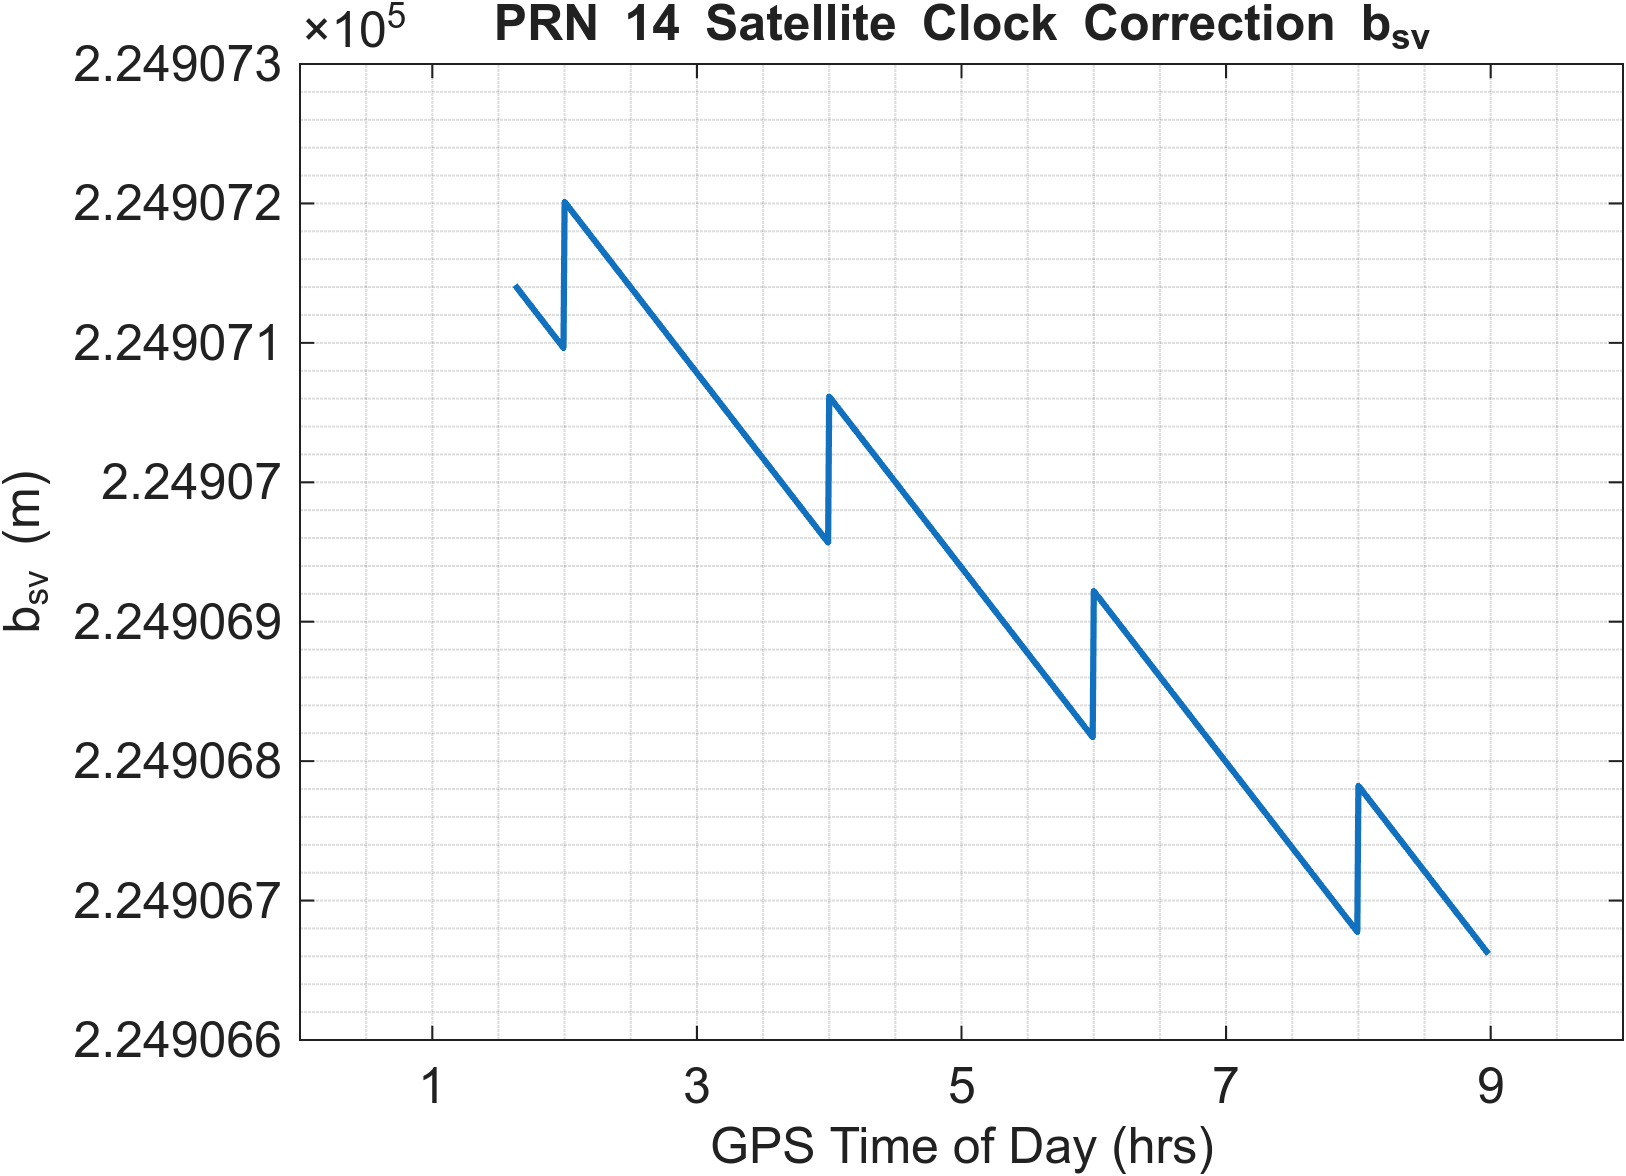
\includegraphics[width=0.6\textwidth]{../MATLAB/figures/HW4/HW4_P2_bsv_PRN14.png}
    \caption{Satellite Clock Correction}
    \label{fig:Satellite Clock Correction}
\end{figure}

\hspace*{2em}Taking a look at Figure \ref{fig:Satellite Clock Correction}, we expect to notice a few things. The satellite clock corrections are representing clock offsets that should decrease over time, we can also notice the clock corrections occurring that is correcting GPS time to UTC(USNO) approximately every 2 hours when new broadcast ephemeris is being sent.

\begin{figure}[H]
    \centering
    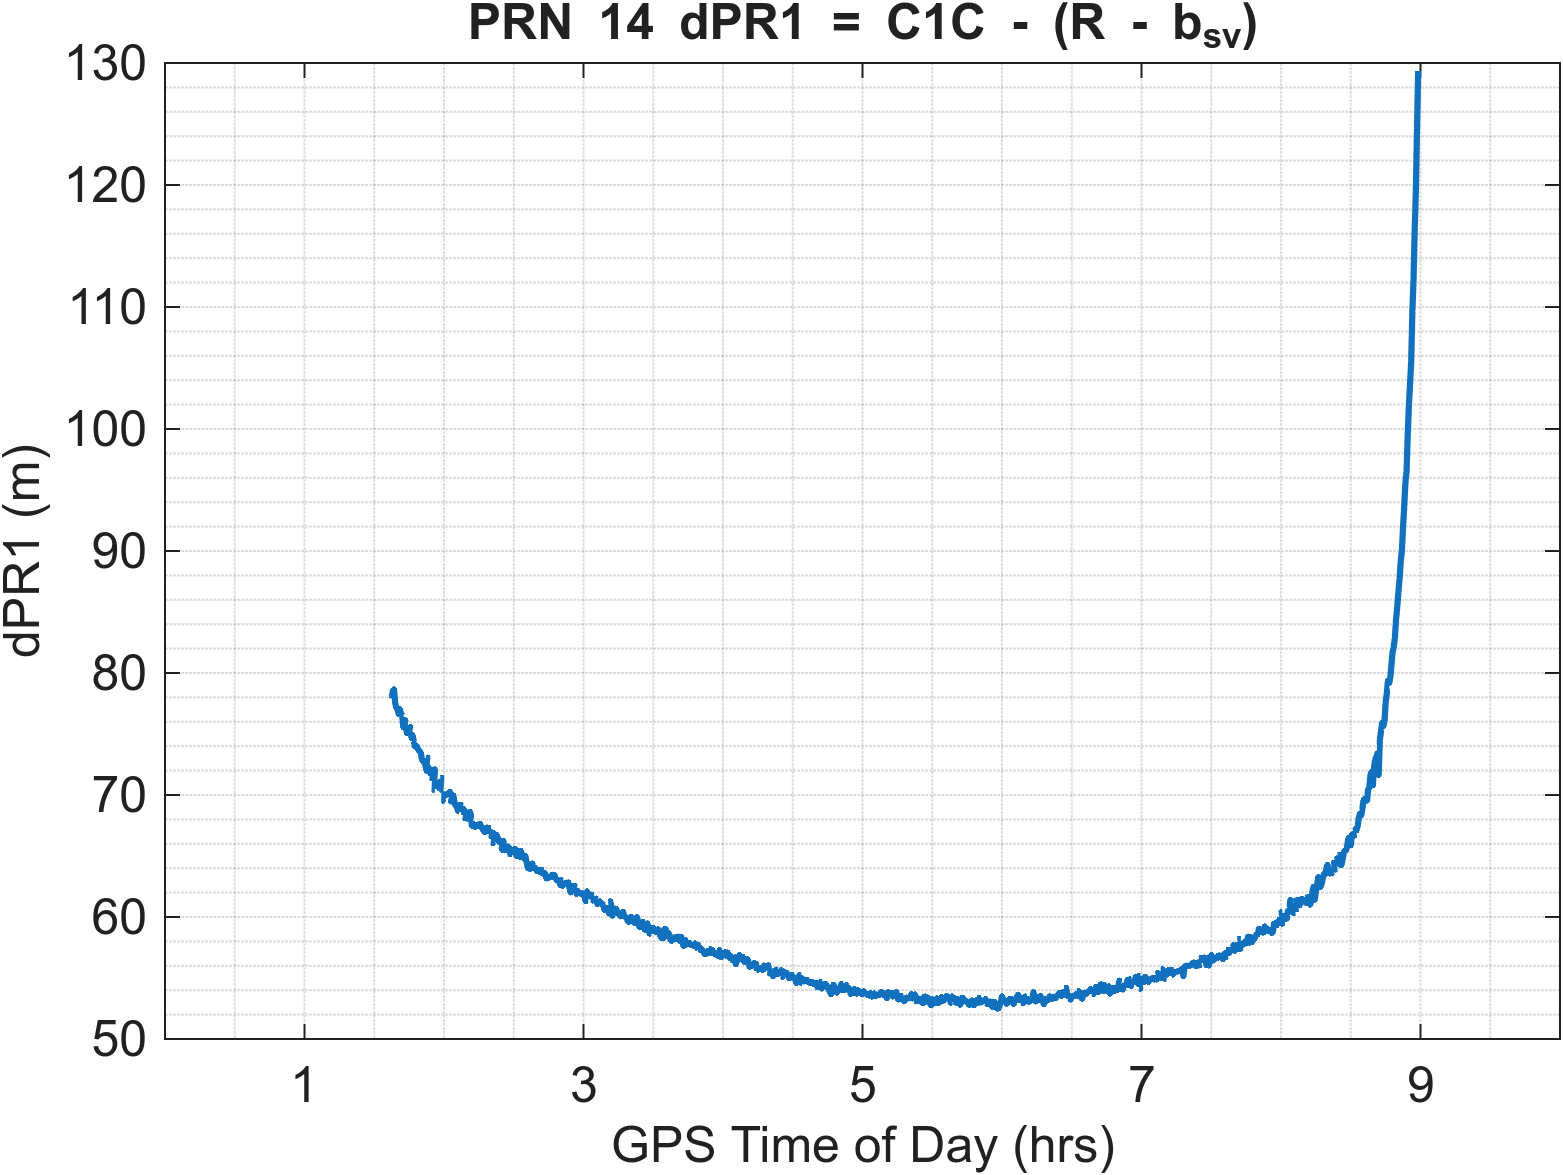
\includegraphics[width=0.6\textwidth]{../MATLAB/figures/HW4/HW4_P2_dPR1_PRN14.png}
    \caption{dPR1 Results}
    \label{fig:dPR1 Results}
\end{figure}

\begin{lstlisting}[language=Matlab]
dPR1 first value: 77.9106 m
dPR1 last value:  129.3488 m
\end{lstlisting}


\newpage
\section*{Problem 3: Relativity}
\begin{figure}[H]
    \centering
    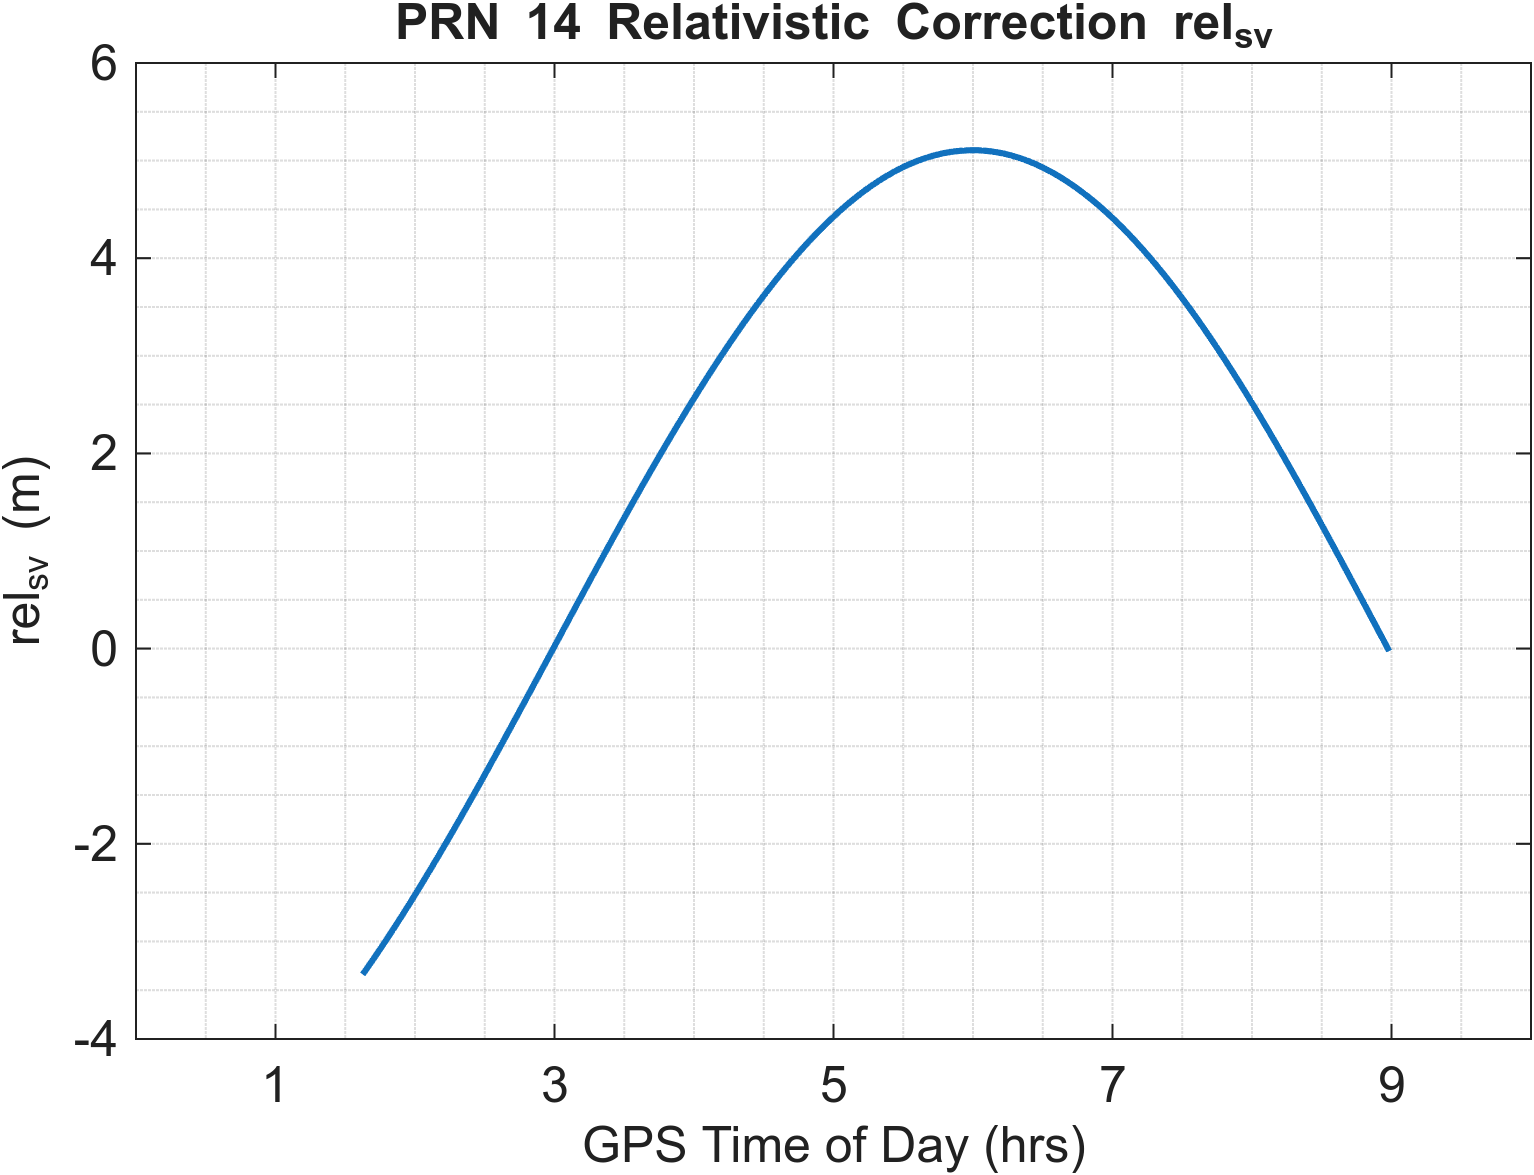
\includegraphics[width=0.6\textwidth]{../MATLAB/figures/HW4/HW4_P3_relsv_PRN14.png}
    \caption{Relativistic Error}
    \label{fig:Relativistic Error}
\end{figure}

\hspace*{2em}In our equation for the relativistic correction it is dependent on $sin(E)$ where E is the eccentric anomaly that tells us where we are in our elliptical orbit. Since we have a $sin(E)$ in our equation and that's the parameter that is not a constant means the graph with time should look like a sine graph.

\begin{figure}[H]
    \centering
    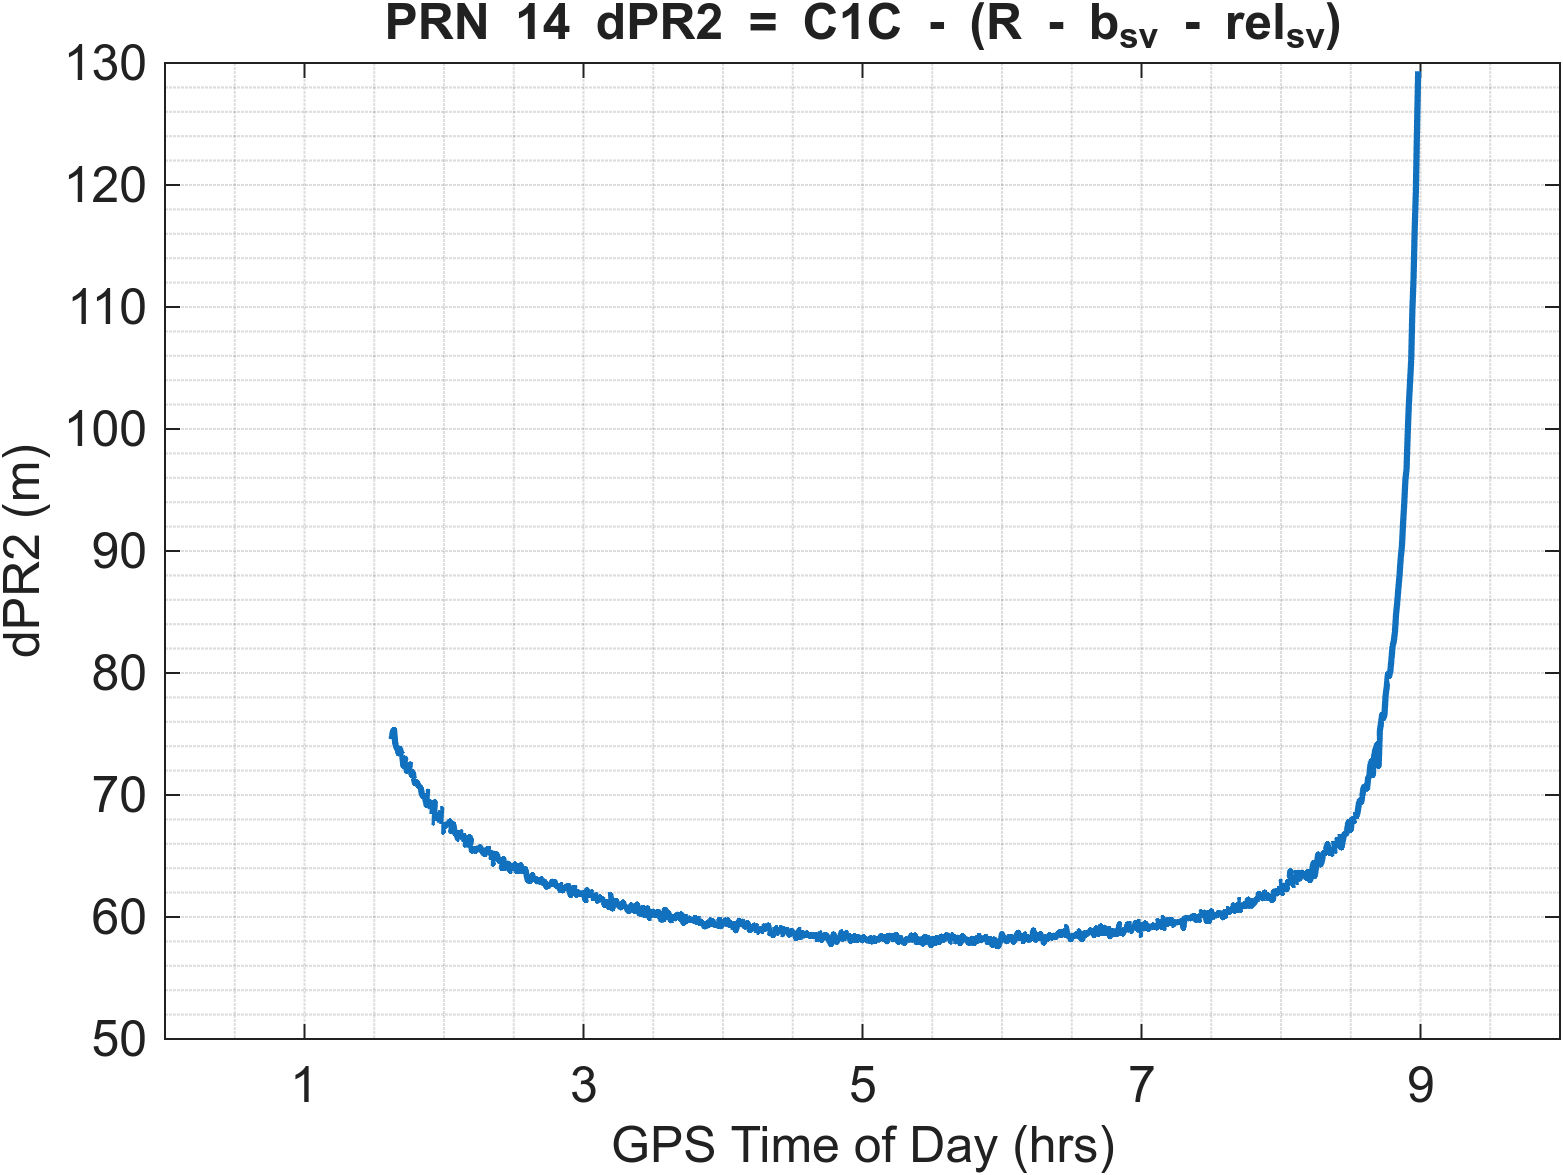
\includegraphics[width=0.6\textwidth]{../MATLAB/figures/HW4/HW4_P3_dPR2_PRN14.png}
    \caption{dPR2 Results}
    \label{fig:dPR2 Results}
\end{figure}

\begin{lstlisting}[language=Matlab]
dPR2 first value: 74.5726 m
dPR2 last value:  129.3236 m
\end{lstlisting}

\newpage
\section*{Problem 4: Troposphere}
\begin{figure}[H]
    \centering
    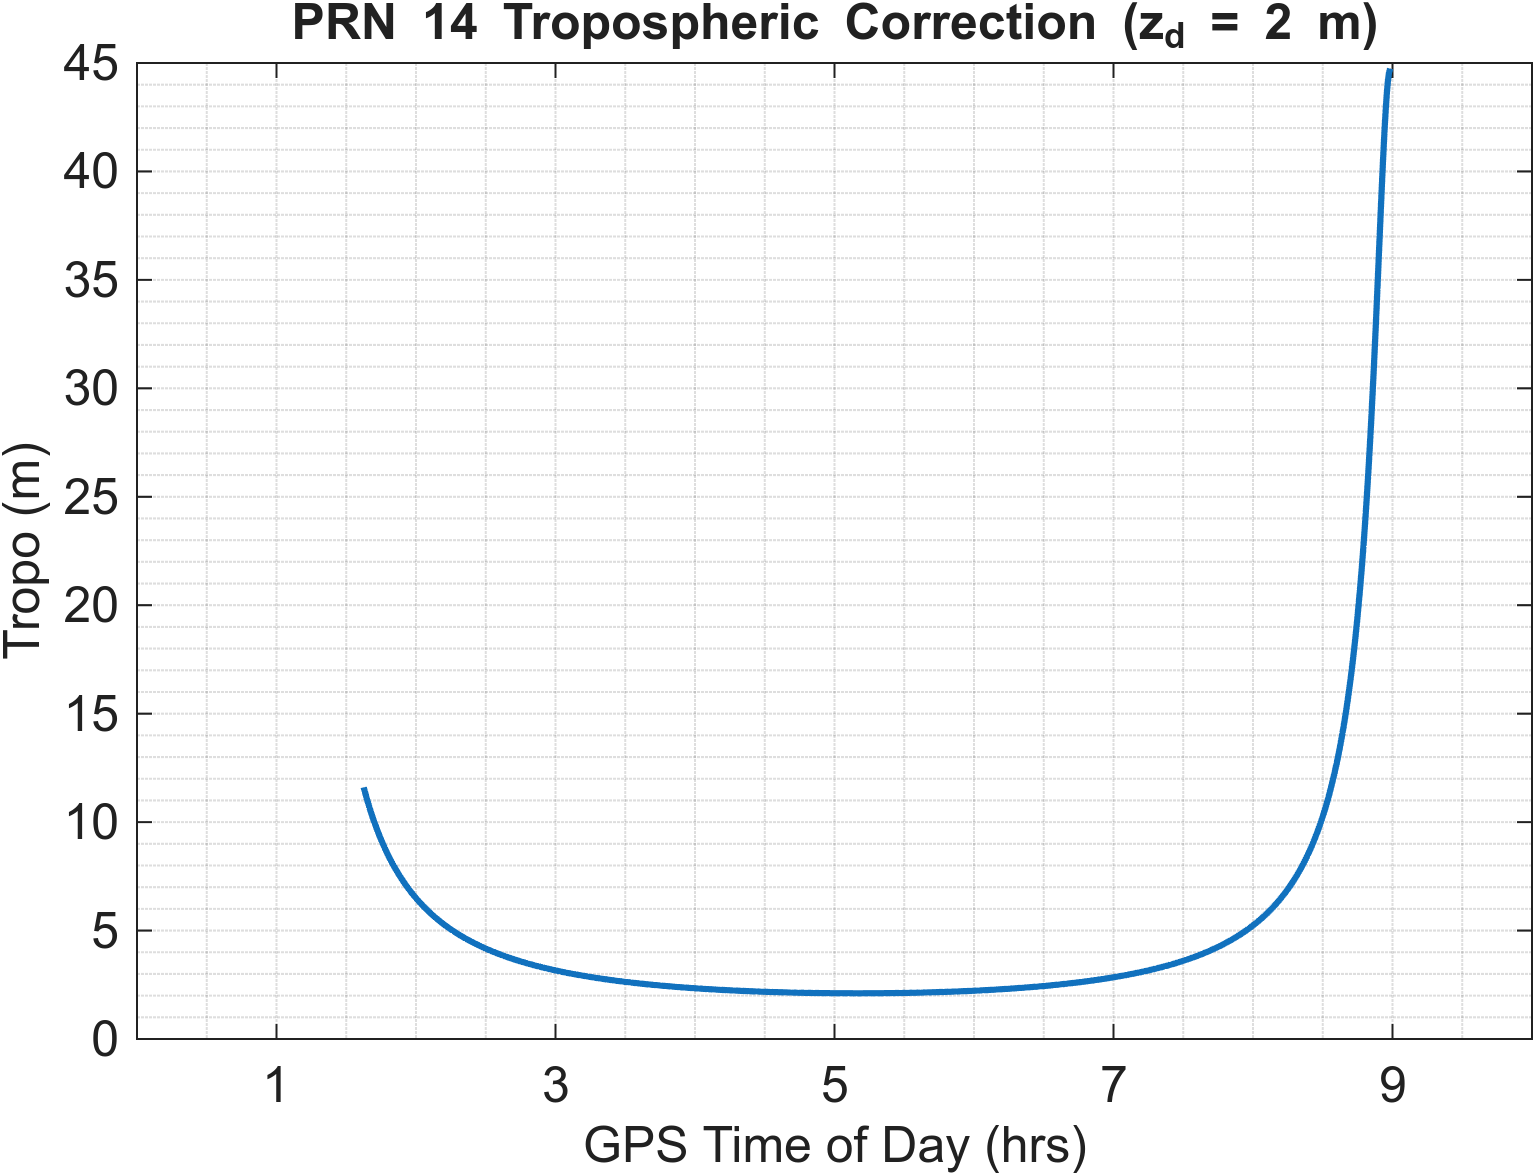
\includegraphics[width=0.6\textwidth]{../MATLAB/figures/HW4/HW4_P4_tropo_PRN14.png}
    \caption{Tropospheric Corrections}
    \label{fig:Tropospheric Corrections}
\end{figure}
\hspace*{2em}When plotting Tropospheric Corrections, we would expect Figure \ref{fig:Tropospheric Corrections} to exhibit characteristics that we would see from tropospheric effects. We would typically see large errors near the start and end of a satellite pass due to the tropospheric delay being proportional to the propagation distance which has a dependence on the incidence angle. 

\begin{figure}[H]
    \centering
    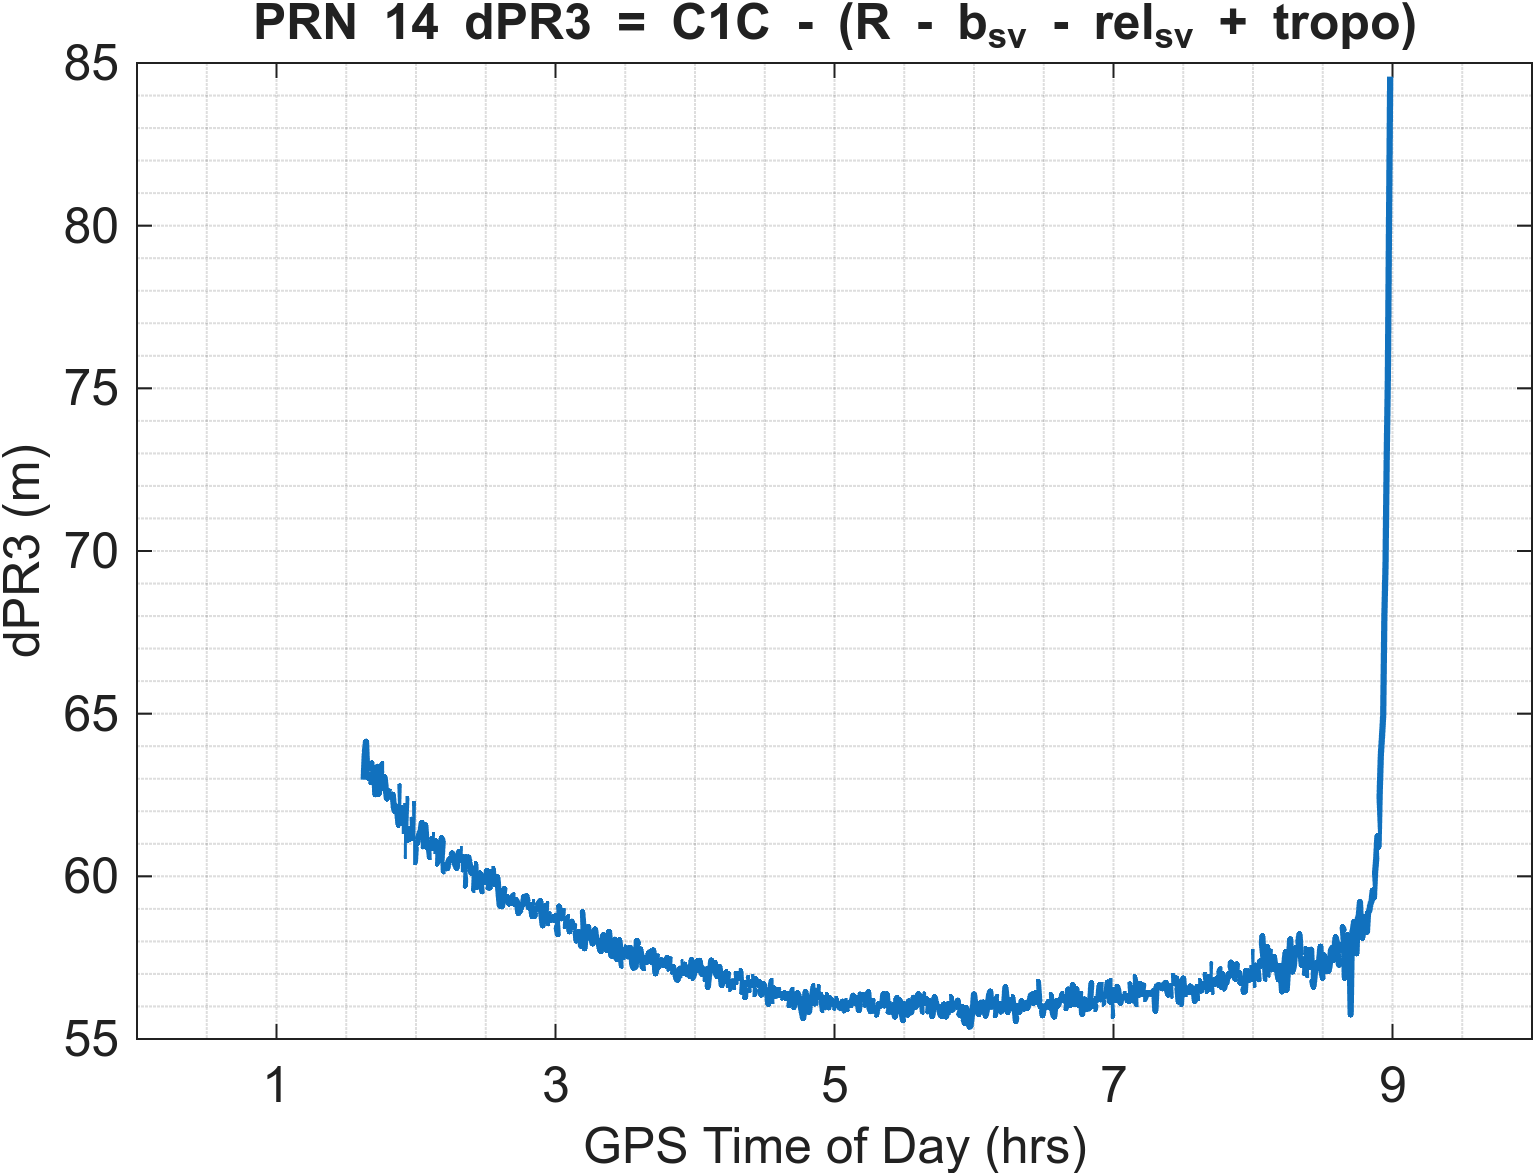
\includegraphics[width=0.6\textwidth]{../MATLAB/figures/HW4/HW4_P4_dPR3_PRN14.png}
    \caption{dPR3 Results}
    \label{fig:dPR3 Results}
\end{figure}

\begin{lstlisting}[language=Matlab]
dPR3 first value: 62.9696 m
dPR3 last value:  84.5804 m
\end{lstlisting}


\newpage
\section*{Problem 5: Ionosphere}
\begin{figure}[H]
    \centering
    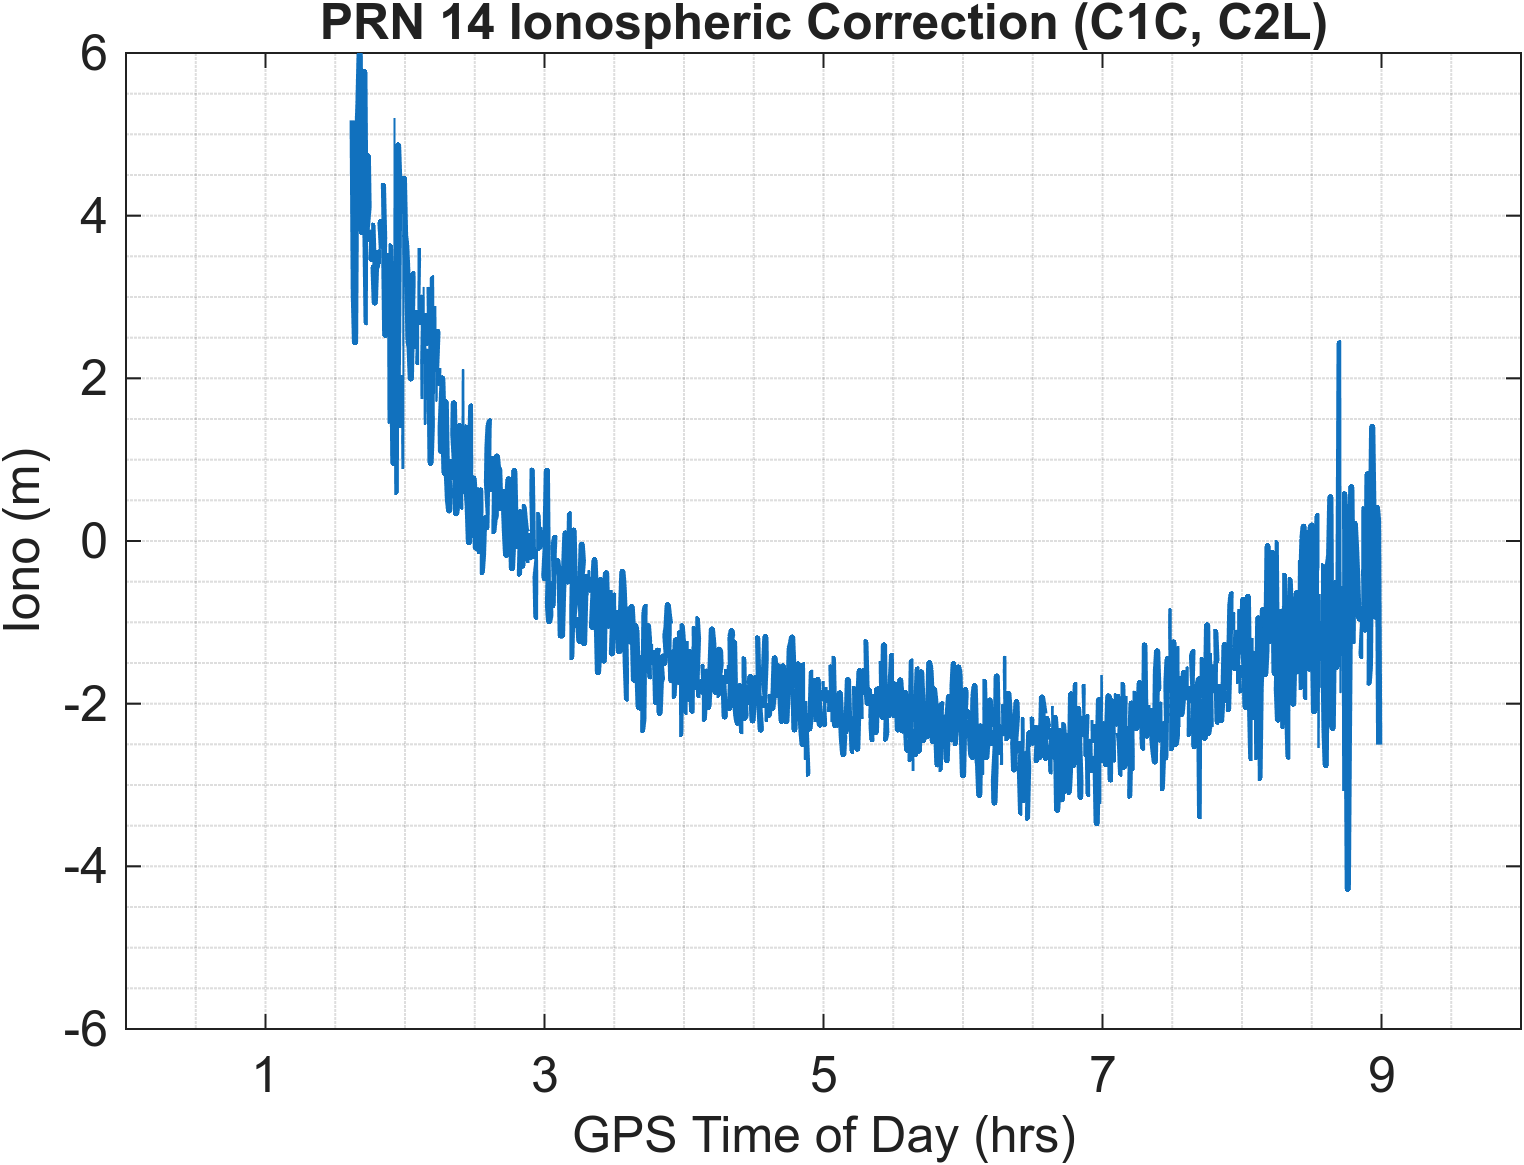
\includegraphics[width=0.6\textwidth]{../MATLAB/figures/HW4/HW4_P5_iono_PRN14.png}
    \caption{Ionospheric Correction (C1C, C2L)}
    \label{fig:Ionospheric Free Pseudoranging}
\end{figure}

\hspace*{2em} We would expect a varying curve since ionosphere is different in regions. We would expect it to look noisy in the signal since we are mixing frequencies and ranges. There should be some positive delay of a handful of meters, where it is larger at the start and end of a pass at lower elevation angles. From dual frequencies being used we would naturally also see a relatively noisy result. 

\begin{figure}[H]
    \centering
    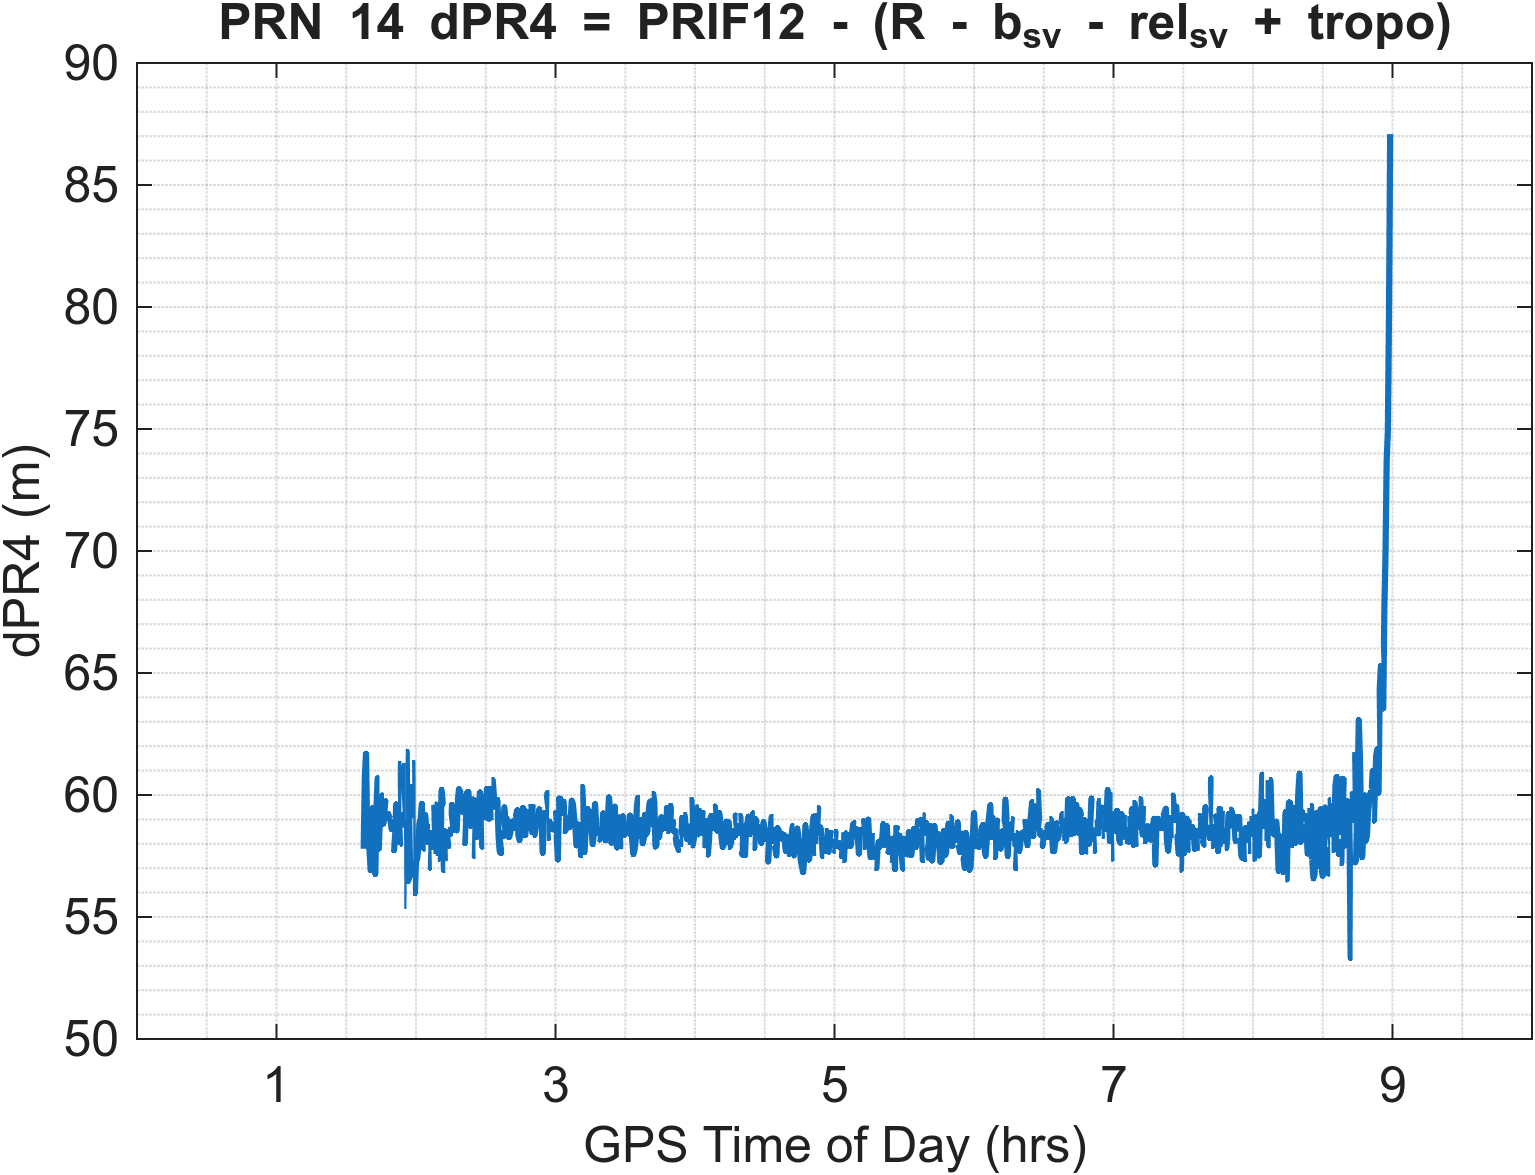
\includegraphics[width=0.6\textwidth]{../MATLAB/figures/HW4/HW4_P5_dPR4_PRN14.png}
    \caption{dPR4 Results}
    \label{fig:dPR4 Results}
\end{figure}

\begin{lstlisting}[language=Matlab]
dPR4 first value: 57.7976 m
dPR4 last value:  87.0845 m
\end{lstlisting}

\newpage
\section*{Problem 6: Discussion}
\begin{figure}[H]
    \centering
    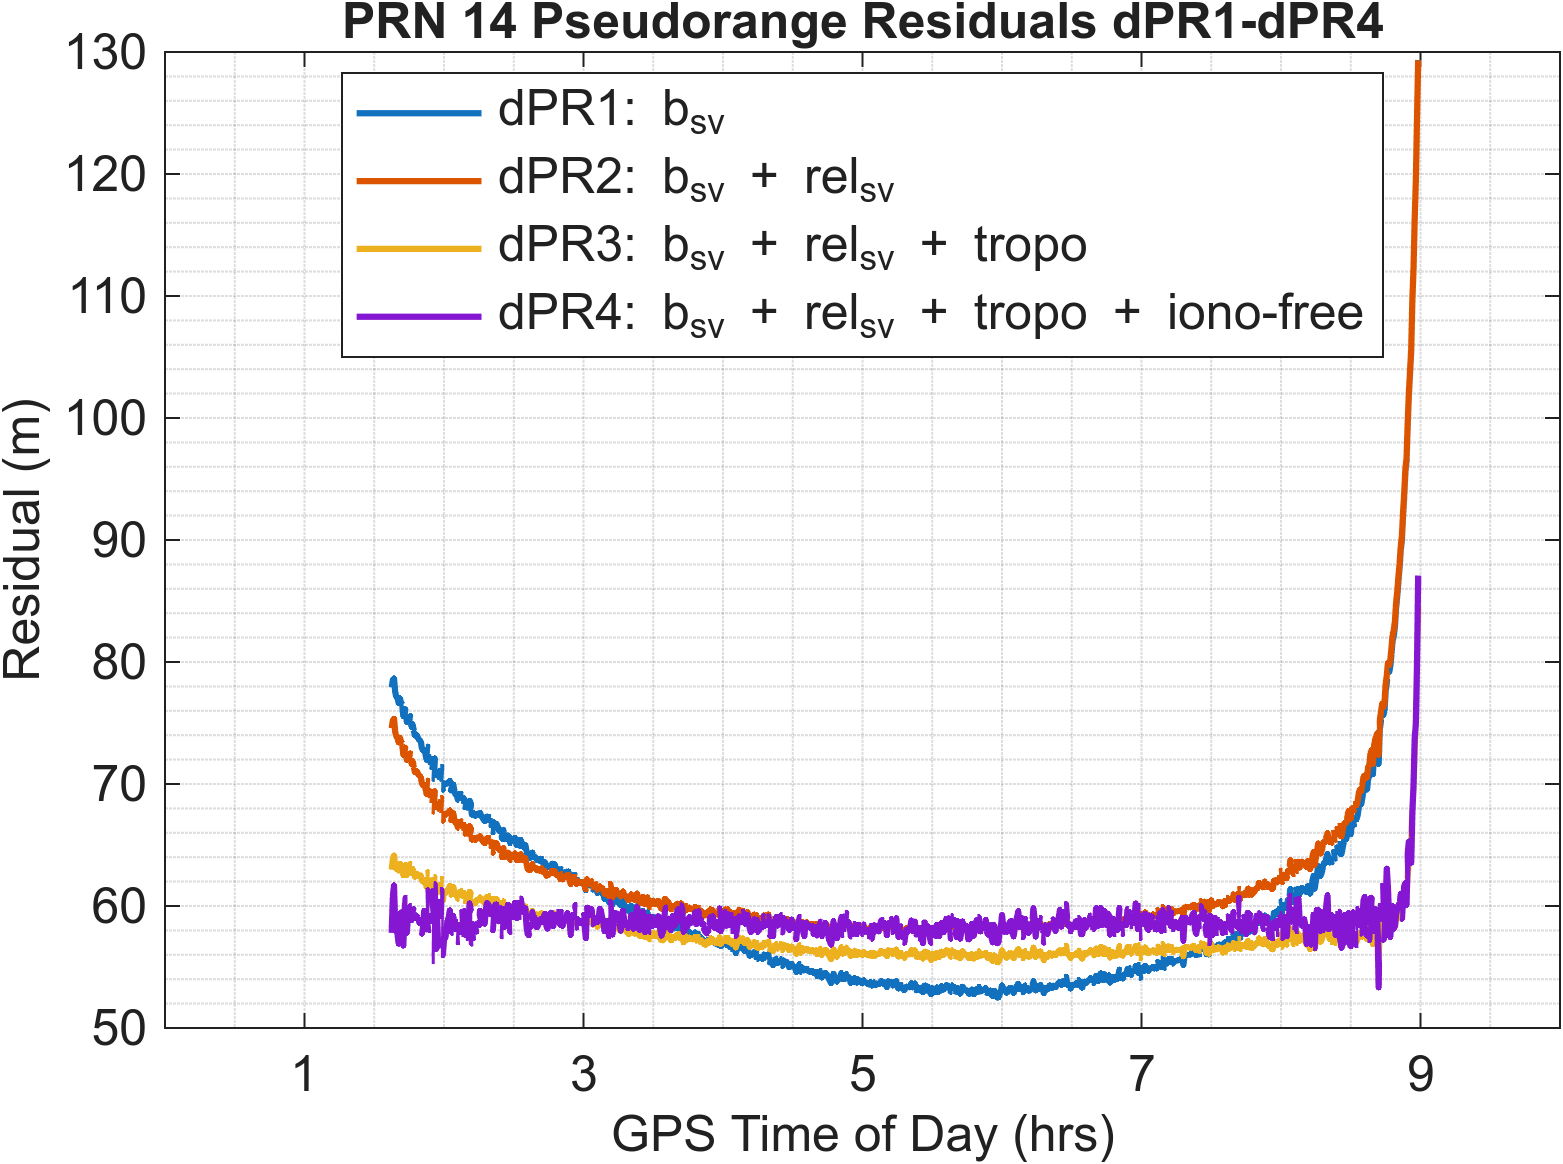
\includegraphics[width=0.6\textwidth]{../MATLAB/figures/HW4/HW4_P6_all_dPRs.png}
    \caption{All dPR Results}
    \label{fig:All dPR Results}
\end{figure}

\hspace*{2em}Examining the results in Figure \ref{fig:All dPR Results}, we notice the cumulative effect of the corrections on the residuals. Our first correction, dPR1, immediately reduces the residuals by several orders of magnitude, to only tens of meters by accounting for clock bias effects. Accounting for the relativistic error improves the residuals in the middle of the satellite pass and slightly improves the start of the pass by a few meters. Incorporating the tropospheric correction significantly improves the start and end of the pass by 10s of meters as well. Finally, accounting for ionospheric effects makes the residuals much less time dependent, so they remain nearly constant over the pass by a couple meters; it should be noted that since this correction combines measurements on dual frequencies for an ionospheric free model of pseudorange, it also amplifies the measurement noise. We also notice that there is still a relatively constant bias of ~60 meters in this data despite all the corrections that have been applied. This is because of some clock bias being present in the receiver. As discussed in class, NIST's bias in the receiving chain would correspond to ~58 m, which is what we observe in \ref{fig:All dPR Results}.

\newpage
\section*{Problem 7: Multipath}
\begin{figure}[H]
    \centering
    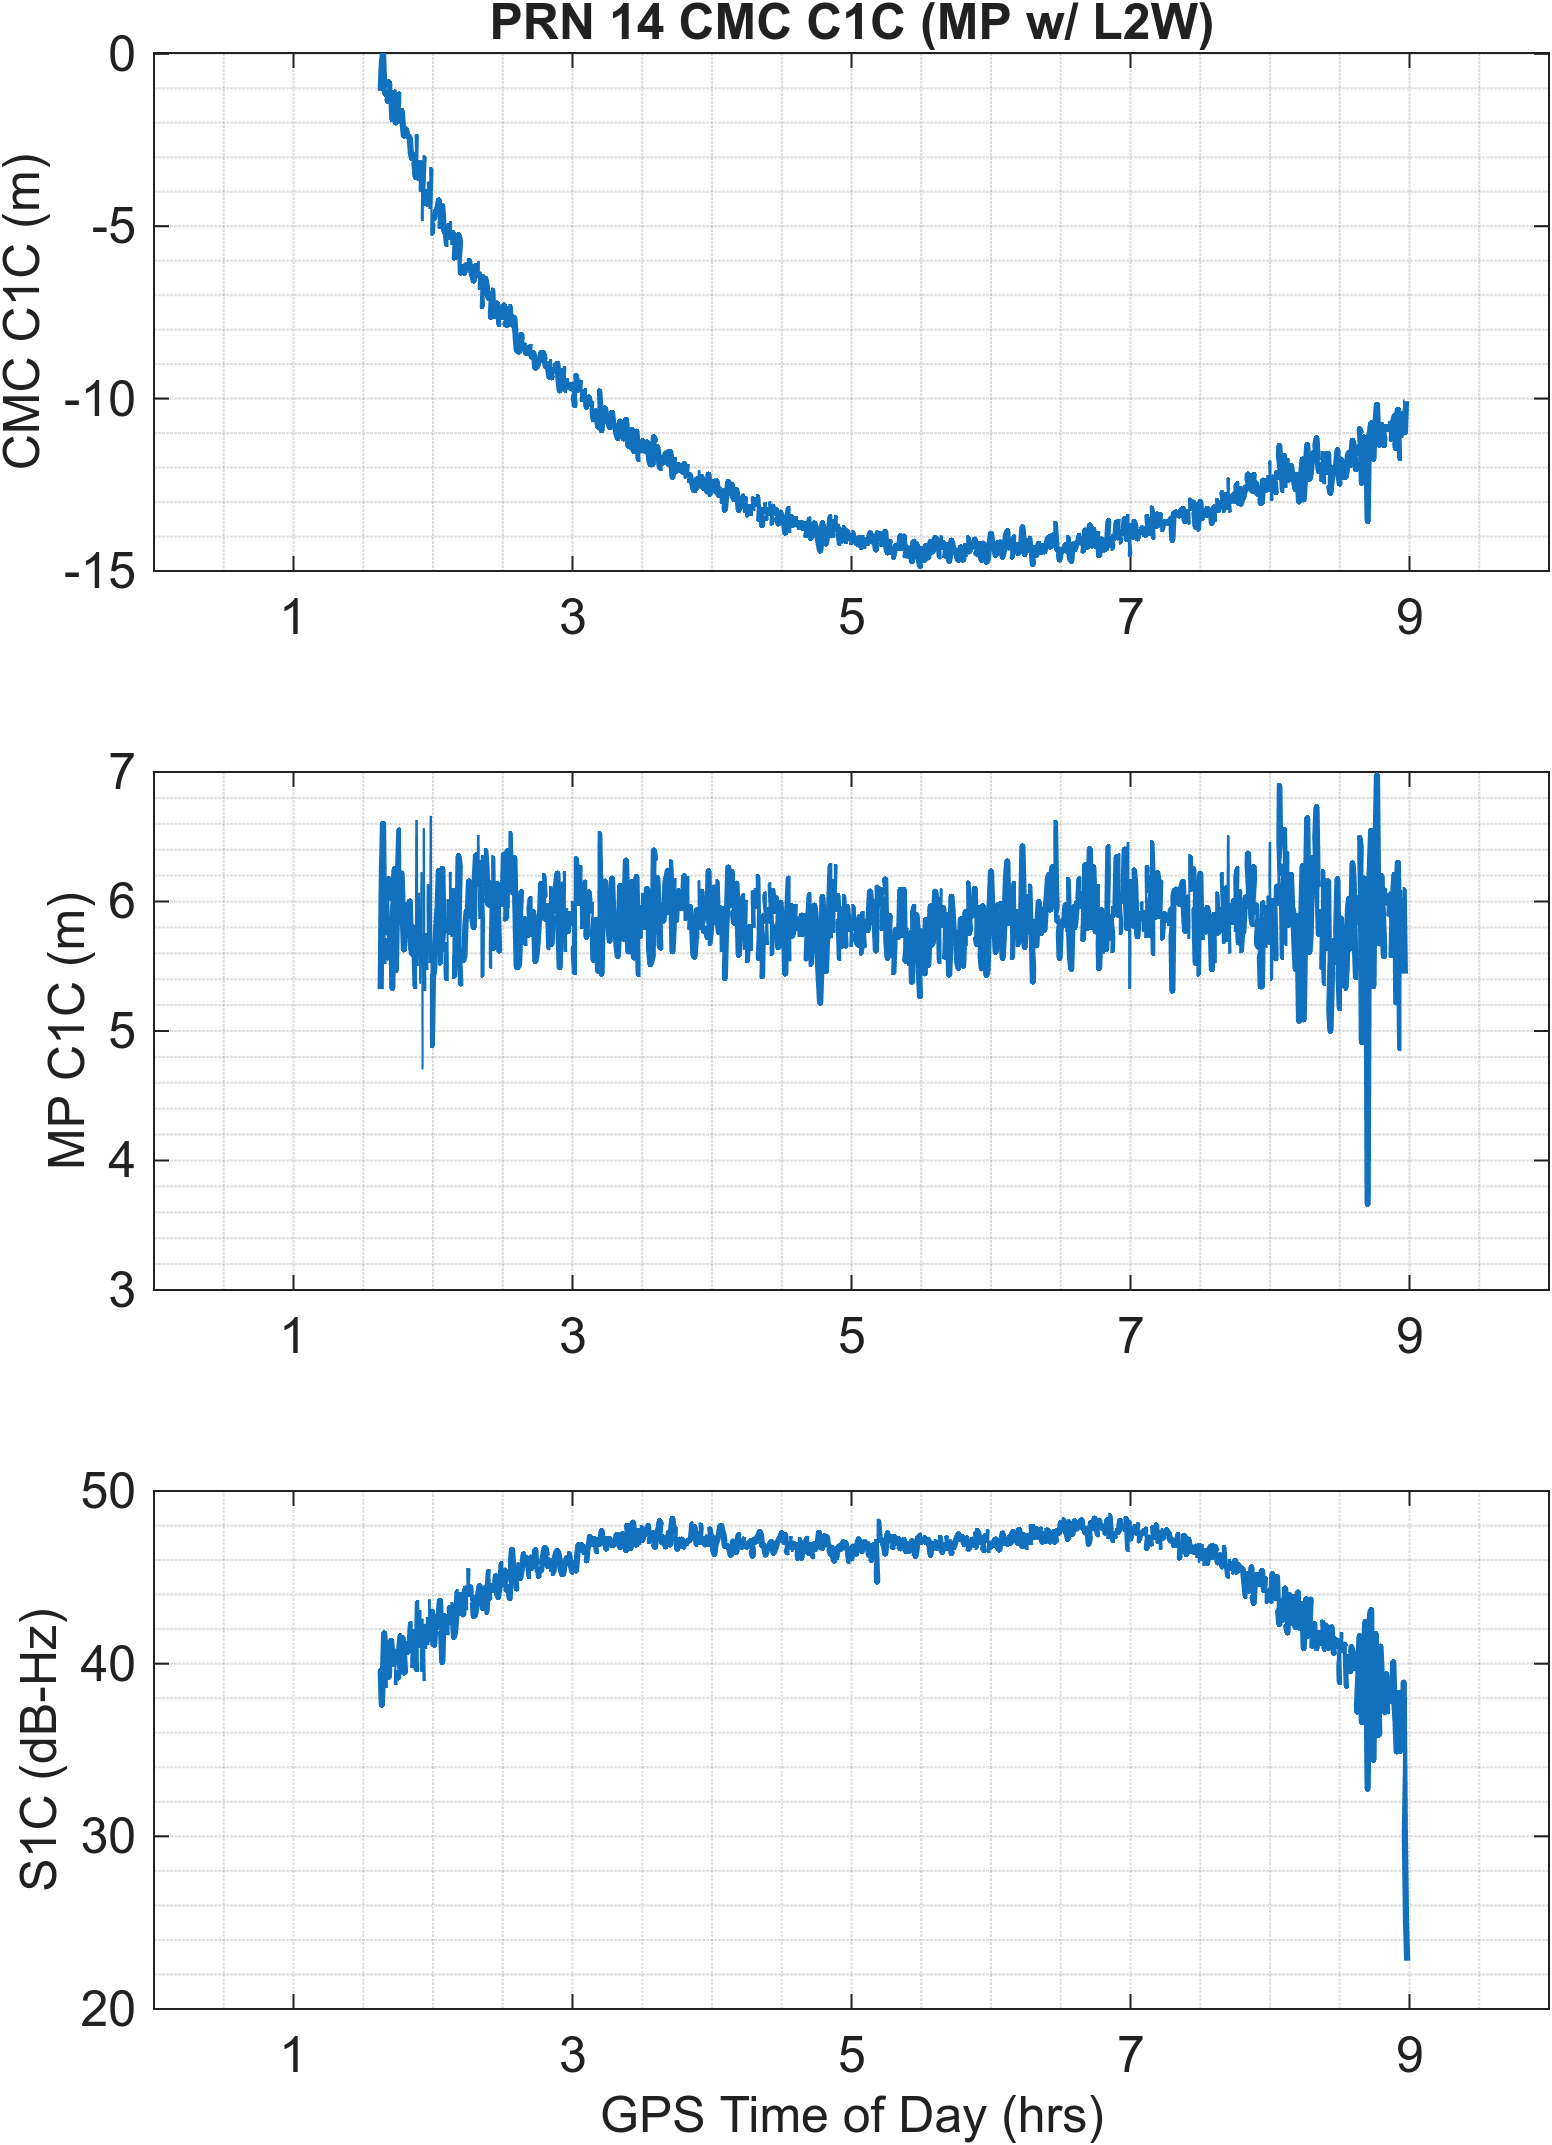
\includegraphics[width=0.6\textwidth]{../MATLAB/figures/HW4/HW4_P7_CMC1.png}
    \caption{CMC1 Multipathing}
    \label{fig:CMC1 Multipathing}
\end{figure}

\begin{figure}[H]
    \centering
    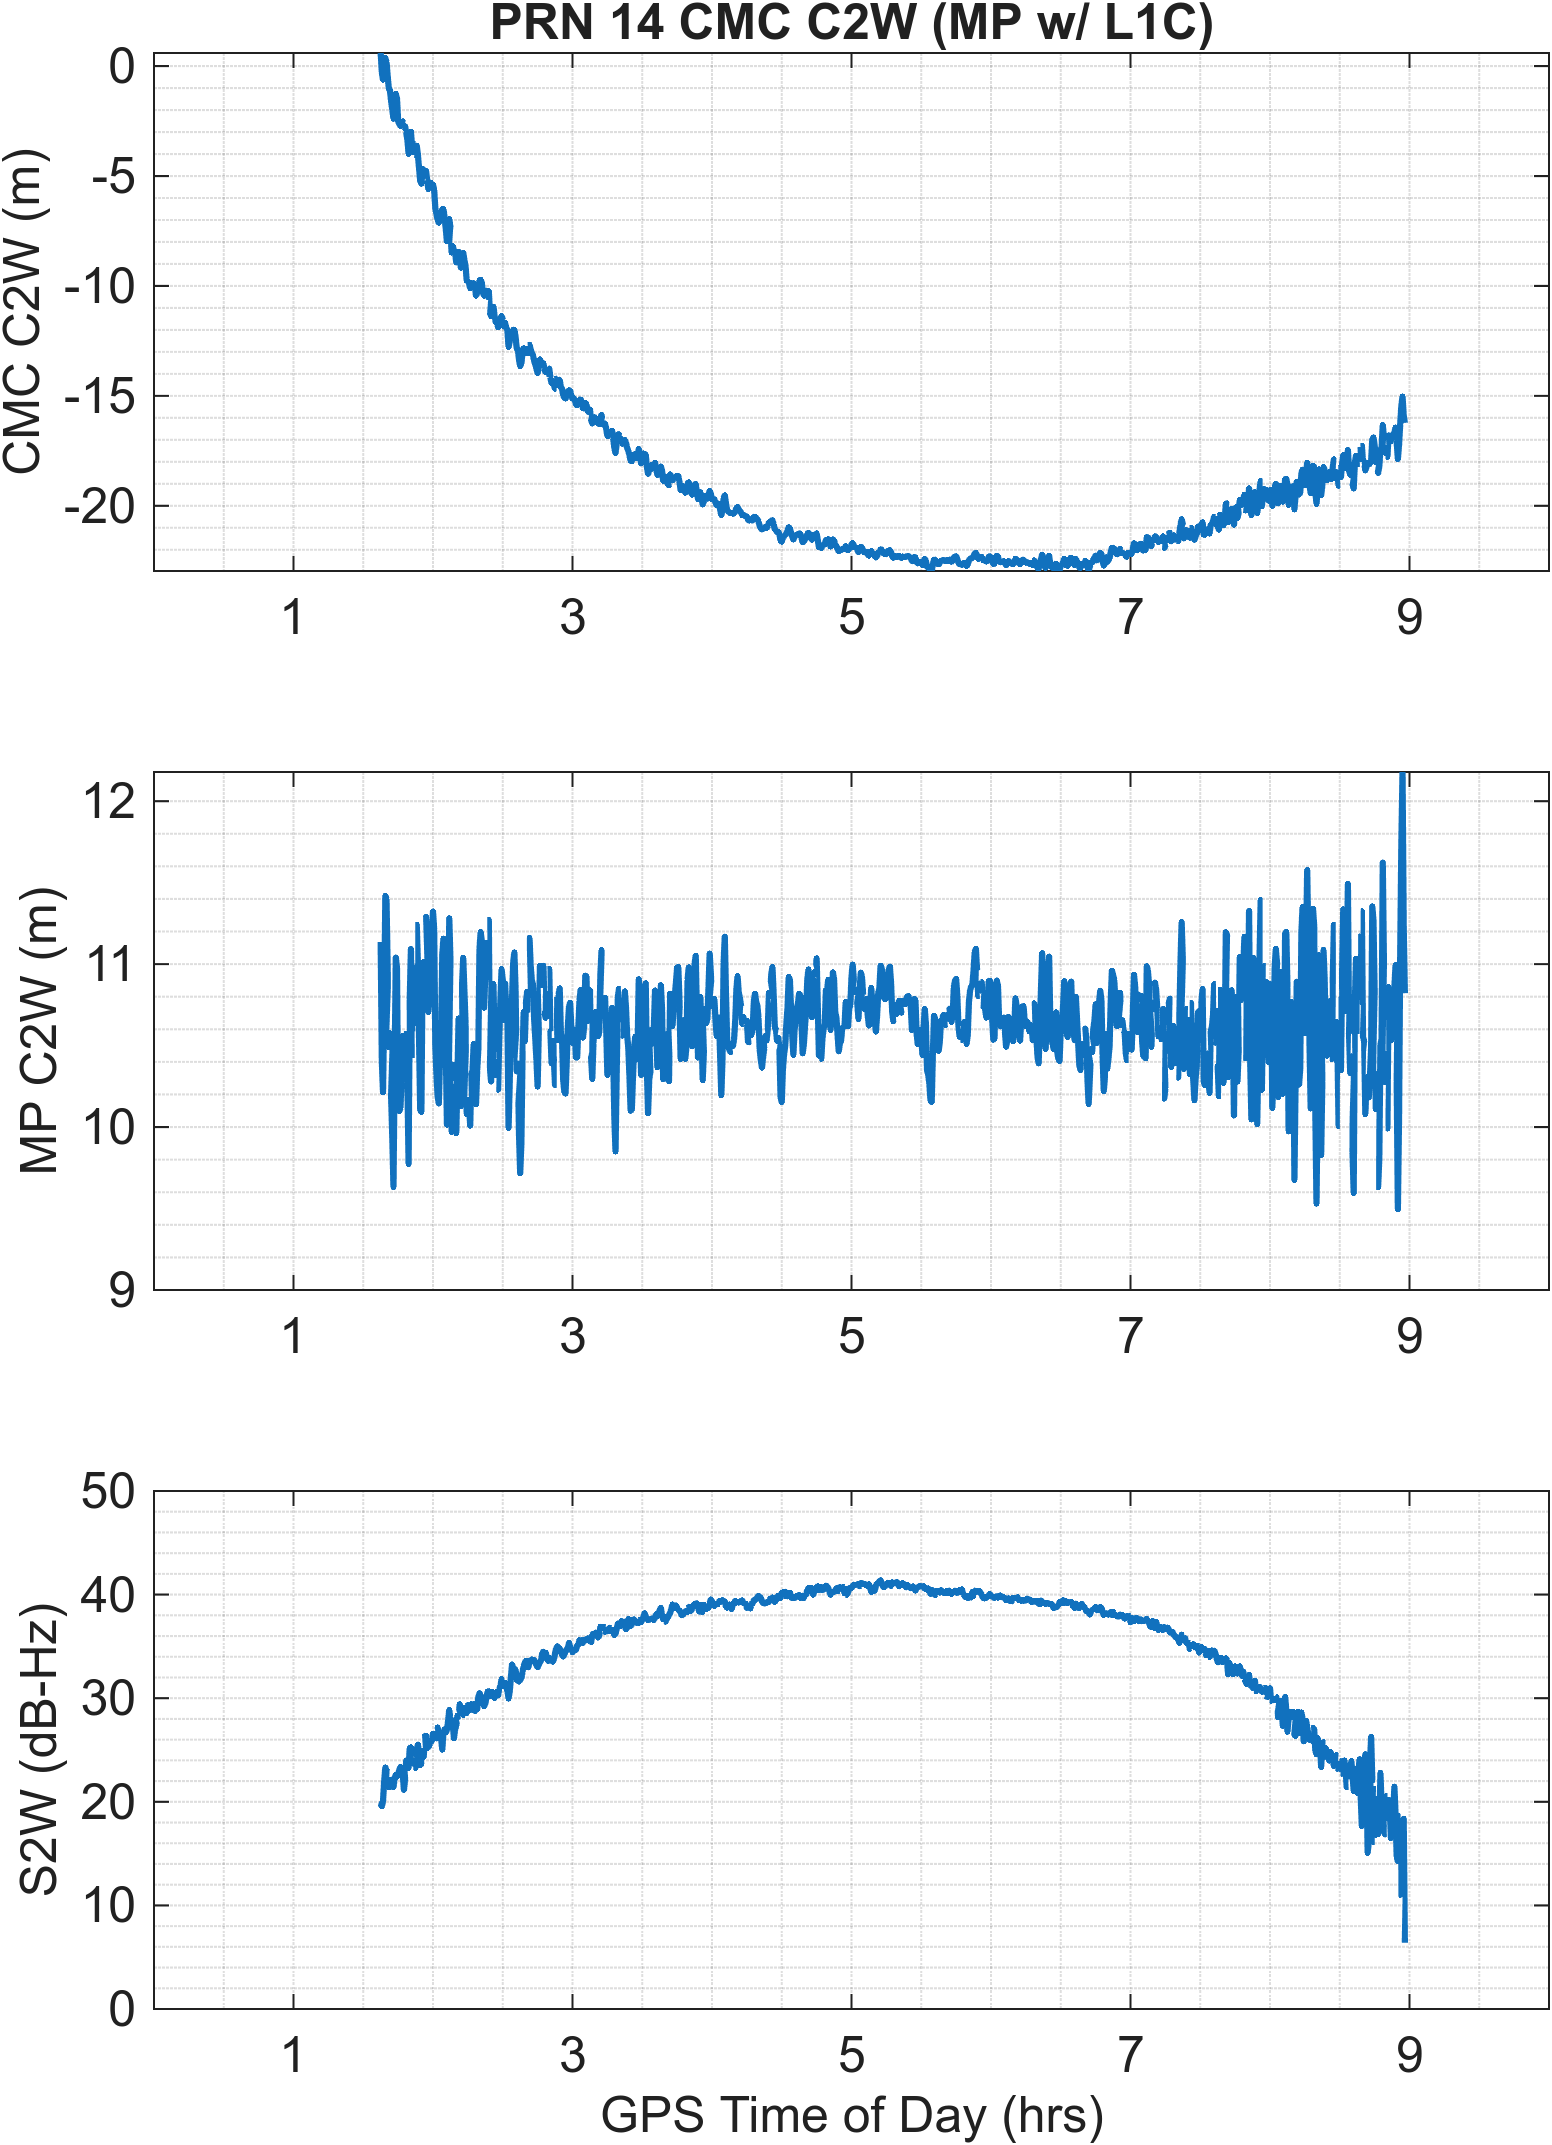
\includegraphics[width=0.6\textwidth]{../MATLAB/figures/HW4/HW4_P7_CMC_C2W.png}
    \caption{C2W Multipathing}
    \label{fig:C2W Multipathing}
\end{figure}

\begin{figure}[H]
    \centering
    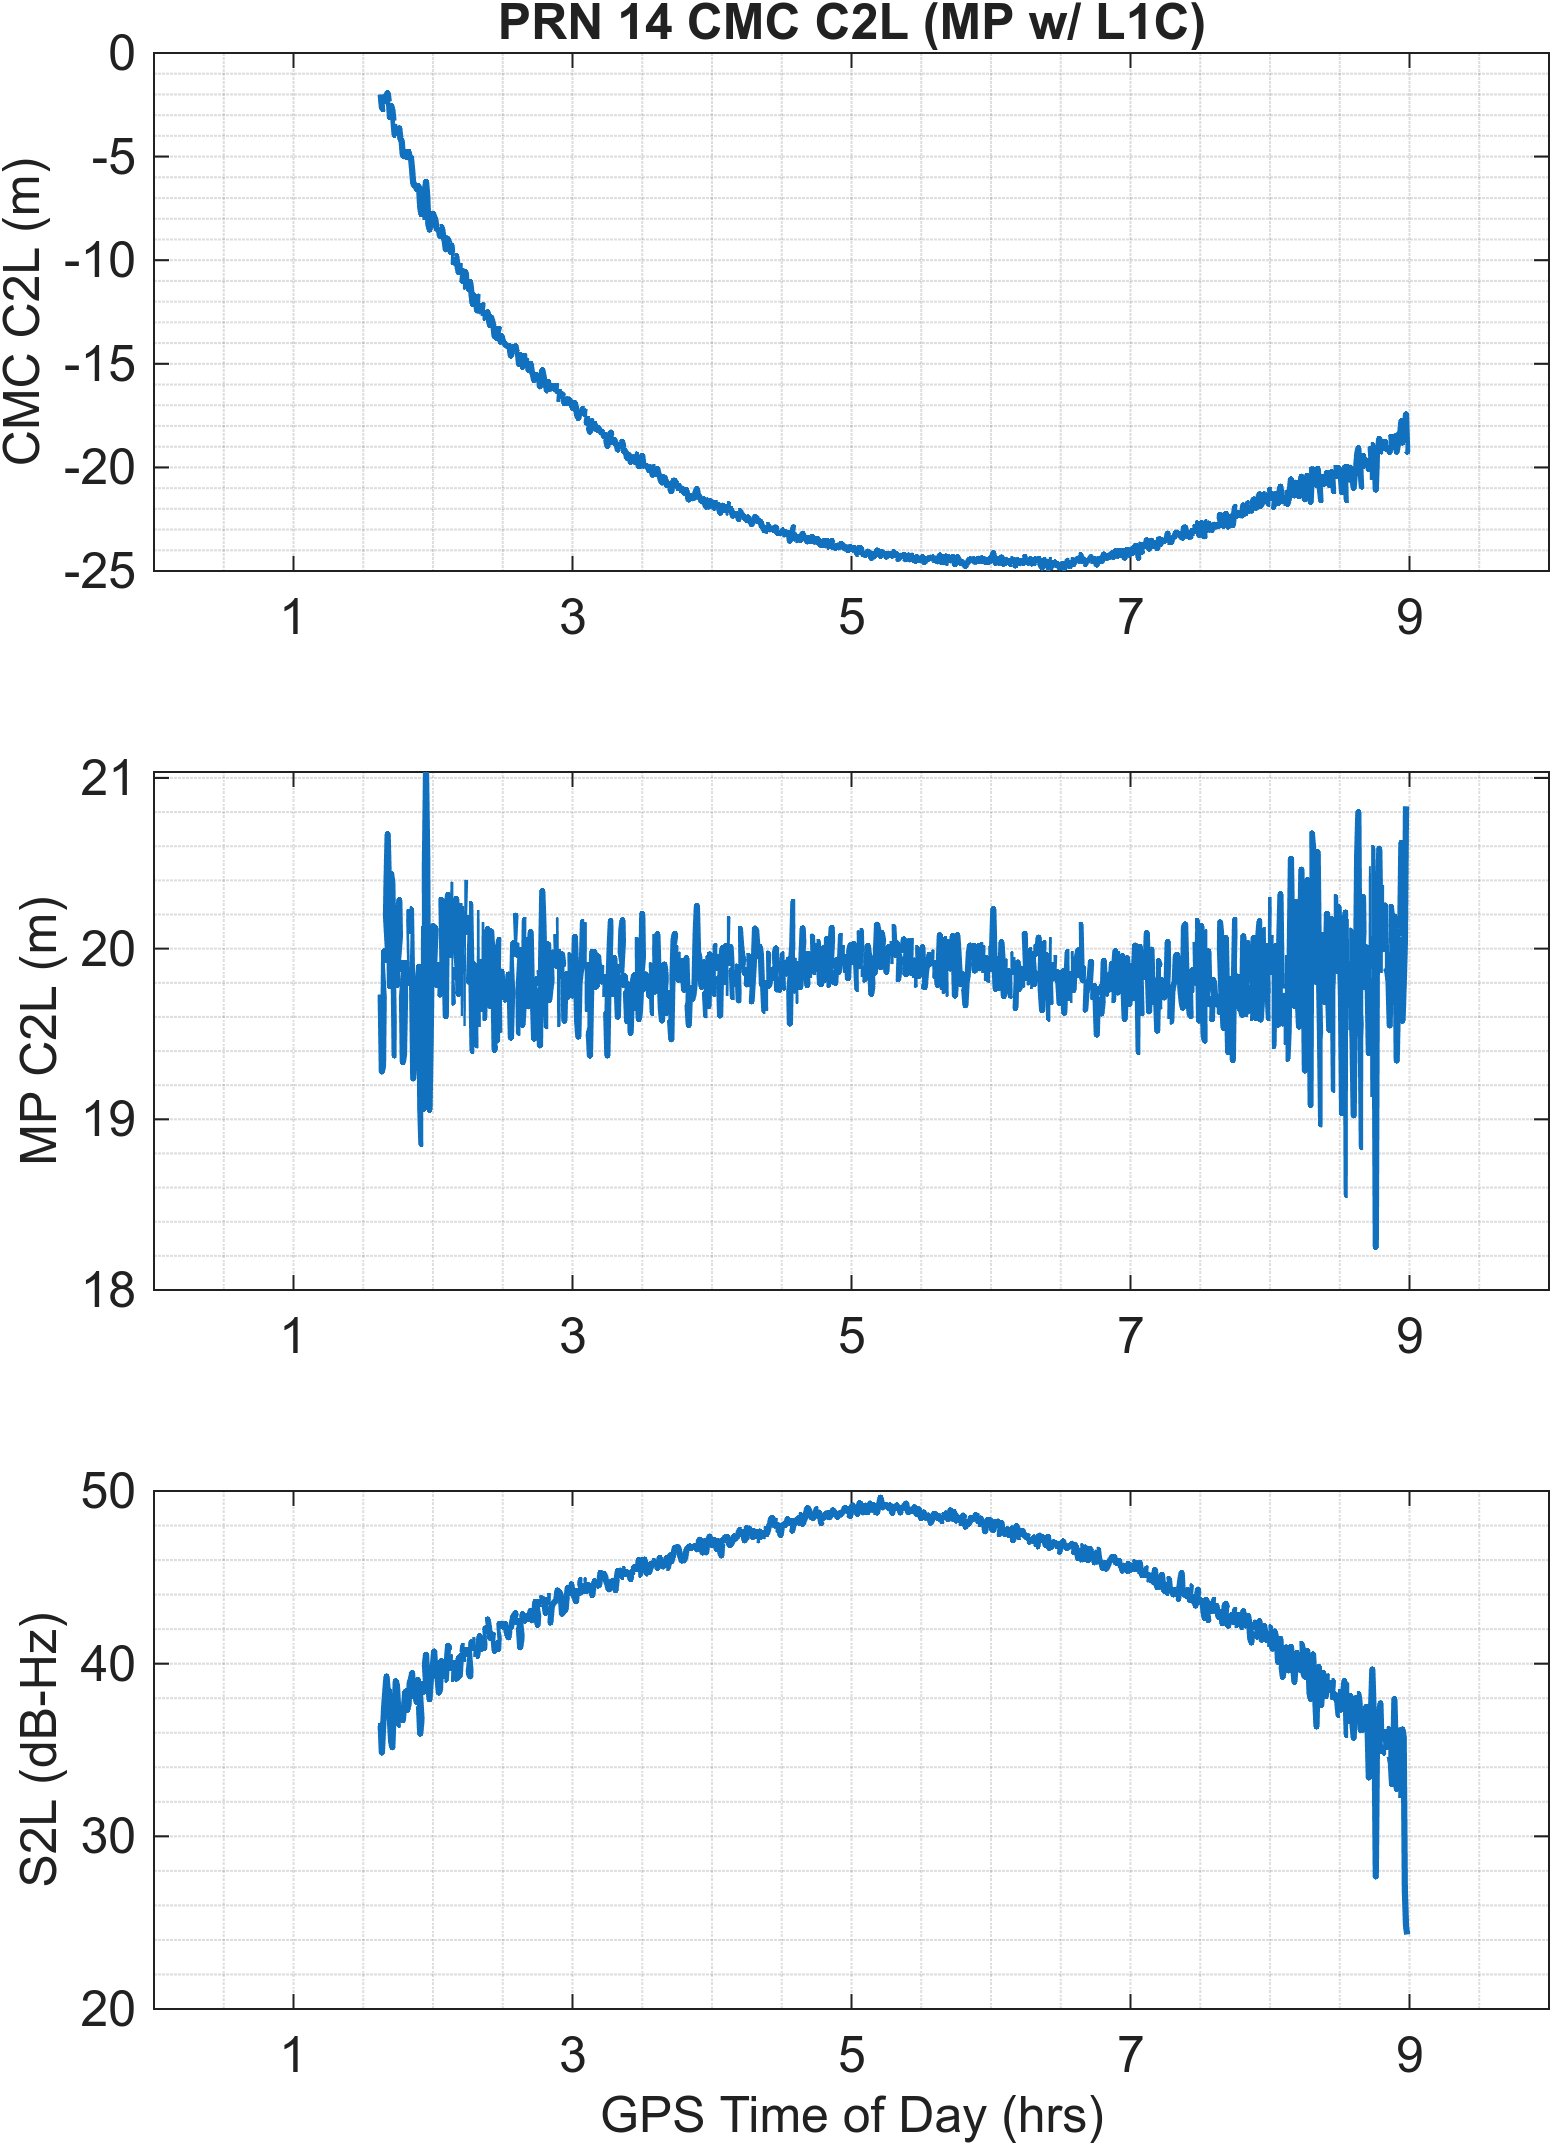
\includegraphics[width=0.6\textwidth]{../MATLAB/figures/HW4/HW4_P7_CMC_C2L.png}
    \caption{C2L Multipathing}
    \label{fig:C2L Multipathing}
\end{figure}

\begin{figure}[H]
    \centering
    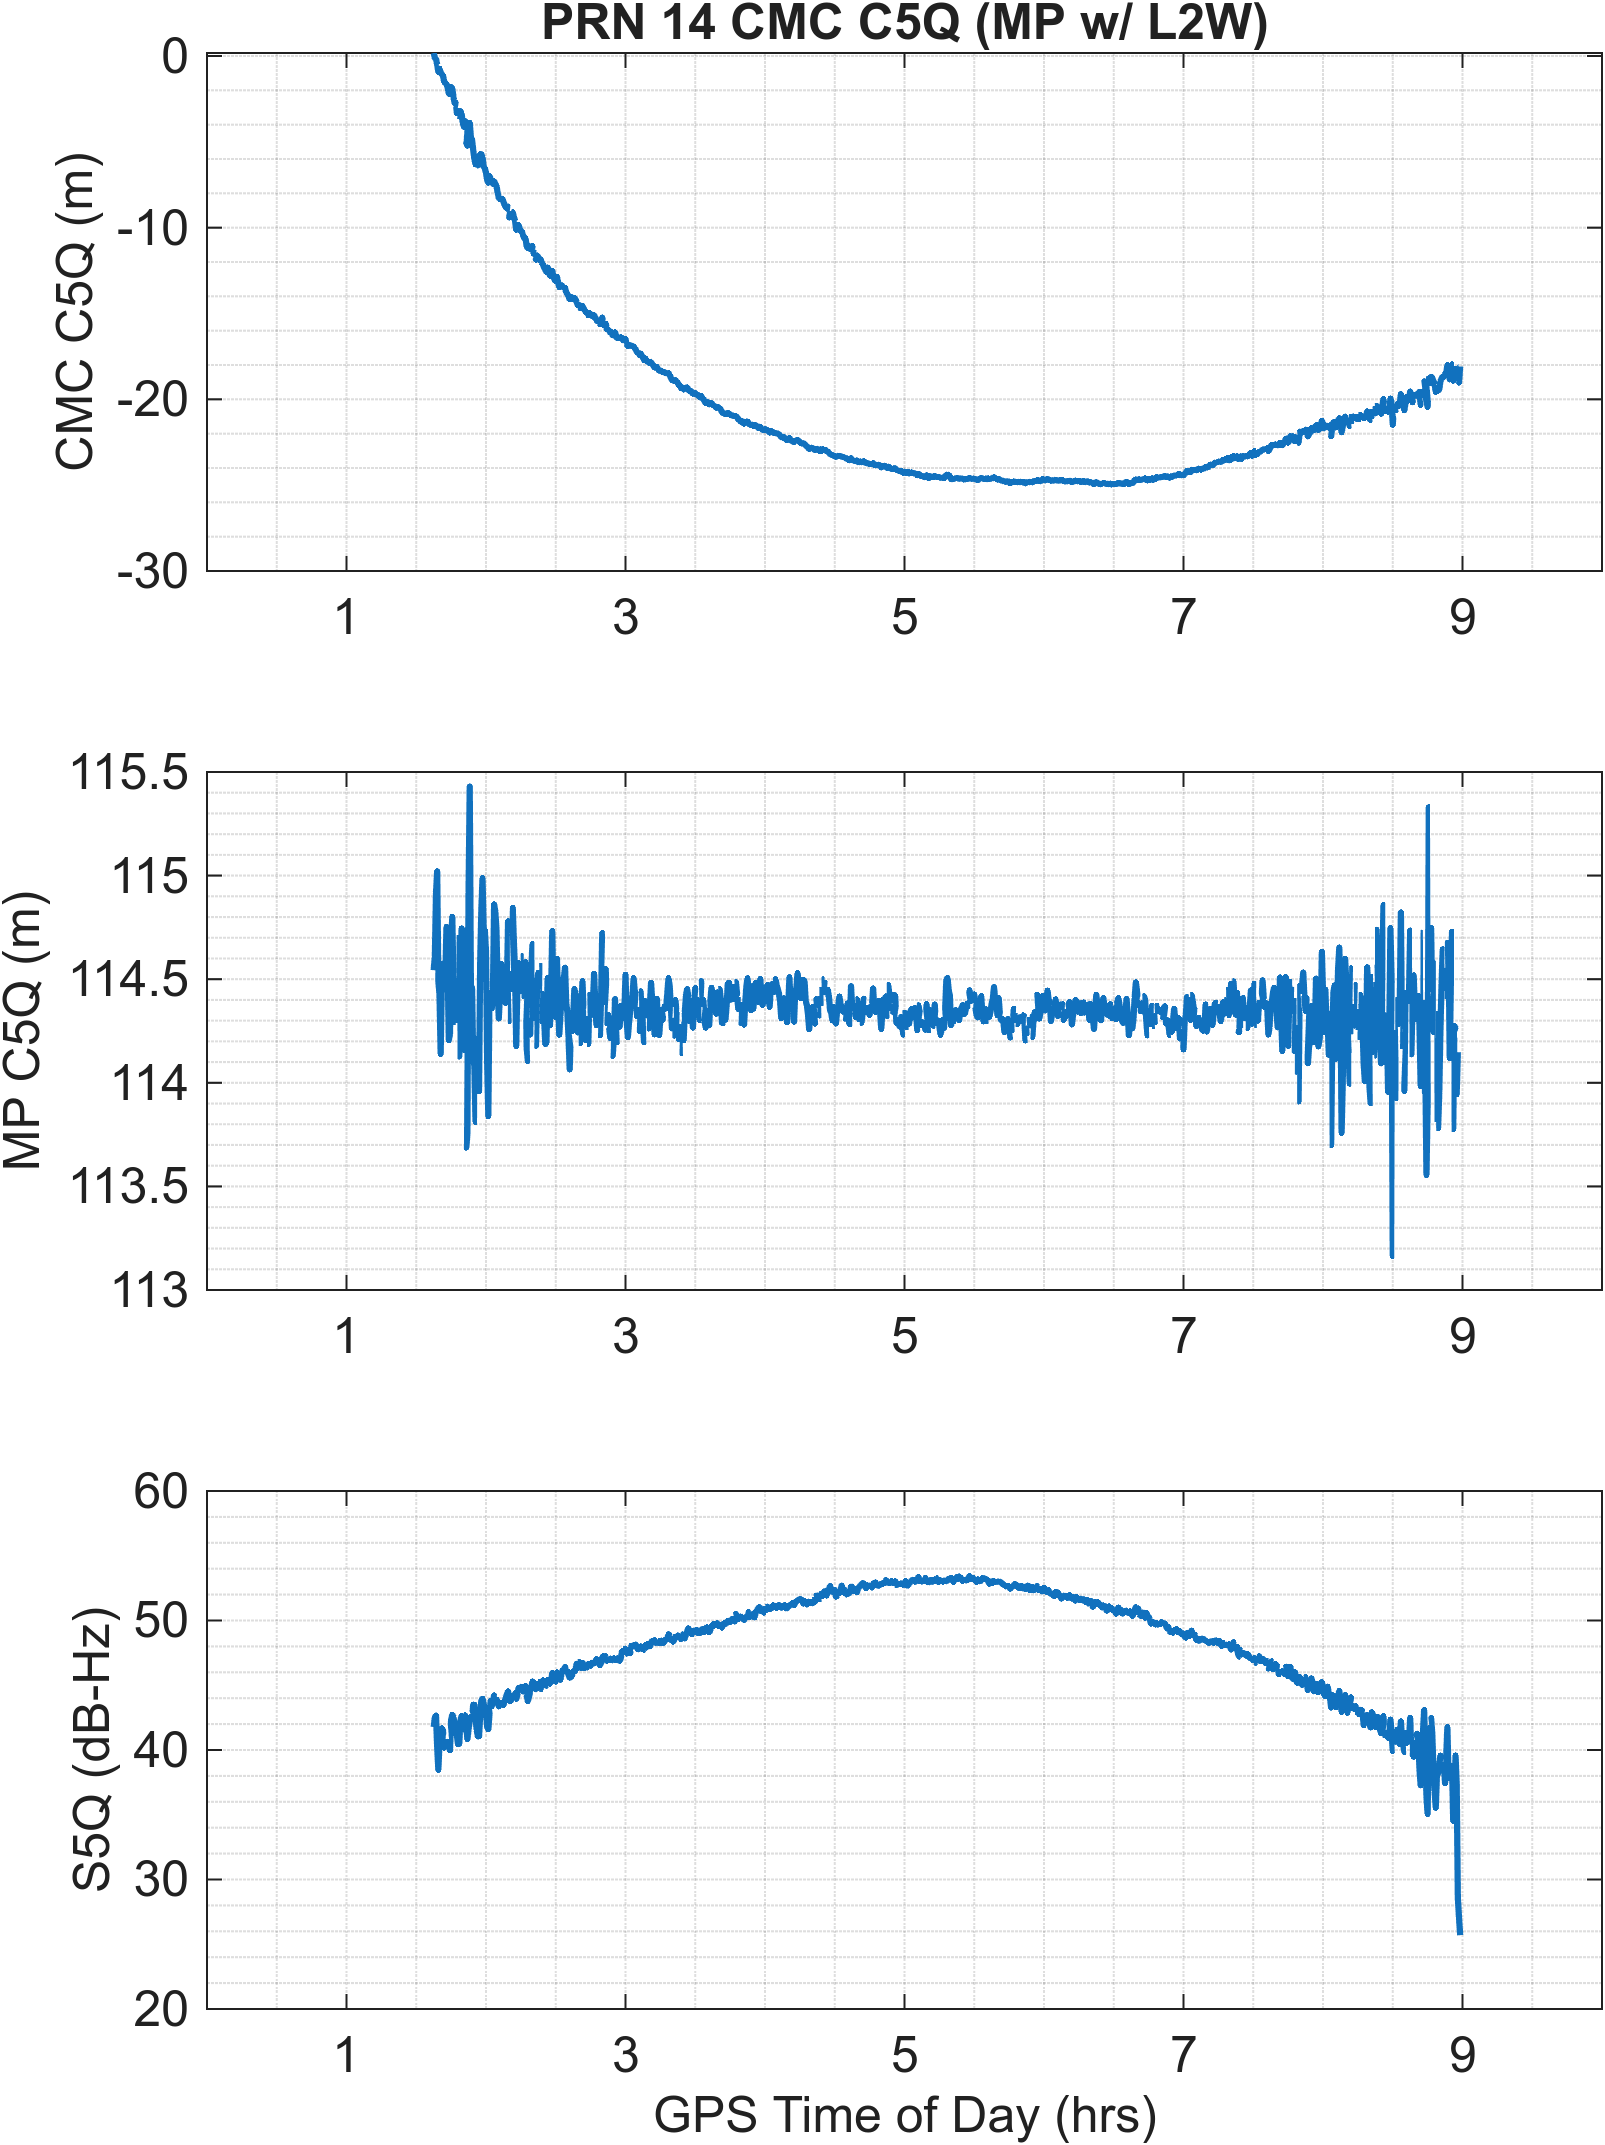
\includegraphics[width=0.6\textwidth]{../MATLAB/figures/HW4/HW4_P7_CMC_C5Q.png}
    \caption{C5Q Multipathing}
    \label{fig:C5Q Multipathing}
\end{figure}

\begin{figure}[H]
    \centering
    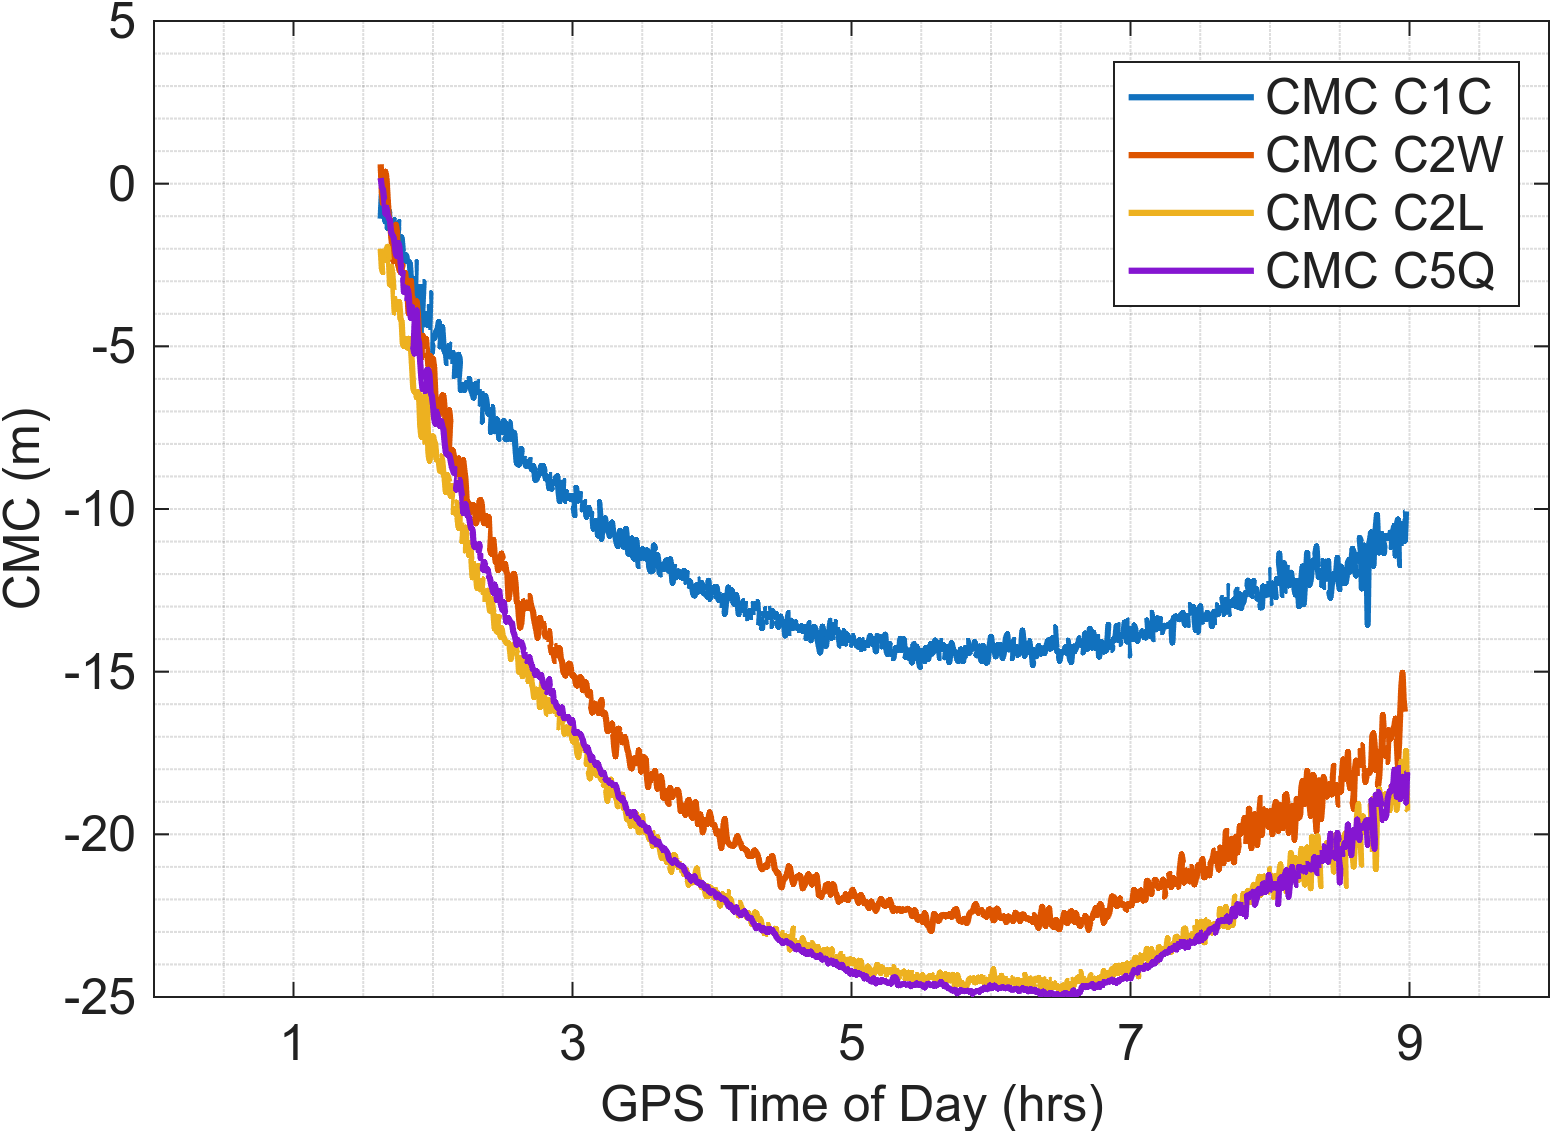
\includegraphics[width=0.6\textwidth]{../MATLAB/figures/HW4/HW4_P7_all_pseudorange.png}
    \caption{All Multipath Pseudoranges}
    \label{fig:All Multipath Pseudoranges}
\end{figure}

\hspace*{2em}Looking at results starting with Figure \ref{fig:CMC1 Multipathing} we can see a lot of noise in C1C once we add multipathing which makes it not a good signal for very crowded cities. The SNR graph for S1C vs time also tells us we should not use this C/A code for positioning in big cities because it's very noisy.


Then from Figure \ref{fig:C2W Multipathing} in the MP C2W graph we see a lot of noise at the edges of the dataset and a smaller amount in the center so it wouldn't be the best positioning item but better than C1C. S2W is much less noisy than S1C with time so it's better for positioning but still not the best.

\hspace*{2em}From Figure \ref{fig:C2L Multipathing} for C2L we see a similar trend to Figure \ref{fig:C2W Multipathing} but we see even more noise reduction when looking at the average signal and not the edges. S2L also is almost smooth so it would be good at positioning.

\hspace*{2em}From Figure \ref{fig:C5Q Multipathing} we can see the edges are a bit noisy but the average signal is almost smooth so this means that C5Q is the best one for multipath defense when positioning. S5Q is the smoothest graph for the SNR vs time so this is another reason why it would be the best one for positioning.

\hspace*{2em}Looking at Figure \ref{fig:All Multipath Pseudoranges} where all the pseudoranges are on one plot we see CMC C5Q and CMC C2L almost overlapping and C1C the furthest from the others which is evidence that C1C is the worst for positioning when multipath is happening and C5Q is the best. This makes sense because C1C is using C/A code and L1 thus it's the oldest one out of the group we are analyzing and it has a broader peak when compared to others like C5Q. C1C is also the first civilian GPS signal thus it must be more crowded so noisier. 

\newpage
\section*{MATLAB Code}
\begin{lstlisting}[language=Matlab]
%% ASEN 5090 GPS/GNSS
%% Justin Le
%% HW4 Main Script
clc;clear;close all

%% Setup
% Reading in rinex
rinexData = rinexread('NIST00USA_R_20262310000_01D_30S_MO.rnx');
rinexDataGPS = rinexData.GPS;

% Read in ephemeris
clean_GPSbroadcast = read_clean_GPSbroadcast('brdc2310.26n', true);

PRN_number = 14;
PRN_index = rinexDataGPS.SatelliteID == PRN_number;
PRN14_GPS_rinexData = rinexDataGPS(PRN_index,:);
PRN14_GPS_rinexData(1,:) = []; % Kill first data point says Axelrad

% Reading in sp3
sp3 = read_sp3('IGS0OPSFIN_20262310000_01D_15M_ORB.SP3');
satPRN = extract_sp3_prn(sp3);


[NIST_GPS_week, NIST_GPS_TOW] = utc2gpstime(PRN14_GPS_rinexData.Time);

NIST_ECEF = [-1288398.567 -4721696.932 4078625.350];

ephem_time_s = NIST_GPS_week.*604800 + NIST_GPS_TOW;
ephem_time_hr = mod(NIST_GPS_TOW, 86400)/3600;

gap_idx = [false; diff(ephem_time_s) > 1.5*median(diff(ephem_time_s))];

% Expected range corrected for light-time and Earth rotation
[R_expected, AZ_expected, EL_expected] = compute_expected_range(clean_GPSbroadcast, NIST_GPS_week, NIST_GPS_TOW, PRN_number, NIST_ECEF);
R_expected(gap_idx) = NaN;

% Find NIST time in hours
NIST_HR = NIST_GPS_week*604800 + NIST_GPS_TOW;

% Plotting satellite clock correction
[health,satPos,satVel,satClkCorr,~,~,relCorr] = eph2pvt2025(clean_GPSbroadcast, [NIST_GPS_week NIST_GPS_TOW], 14);

%% Problem 1
% a. Plot psuedorange and expected ranges, and then residuals
figure()
plot(ephem_time_hr, R_expected, 'LineWidth', 1.5)
hold on
plot(ephem_time_hr, PRN14_GPS_rinexData.C1C, 'LineWidth', 1.5)
xlabel('GPS Time of Day (hrs)')
ylabel('Range (m)')
grid minor
legend('Expected Range R', 'Pseudorange C1C', 'Location', 'best')
title(sprintf('PRN %d C1C Pseudorange and Expected Range', PRN_number))
set(gcf, 'Units', 'inches', 'Position', [0 0 6 4]);
set(findall(gcf, '-property', 'FontSize'), 'FontSize', 12);
set(findall(gcf, 'Type', 'axes'), 'XTick', floor(min(ephem_time_hr)):2:ceil(max(ephem_time_hr)));
exportgraphics(gcf, fullfile('figures', 'HW4', 'HW4_P1_C1C_vs_R_PRN14.png'), 'Resolution', 300);

figure()
plot(ephem_time_hr, PRN14_GPS_rinexData.C1C-R_expected, 'LineWidth', 1.5)
xlabel('GPS Time of Day (hrs)')
ylabel('dPR0 (m)')
grid minor
title(sprintf('PRN %d dPR0 = C1C - R', PRN_number))
set(gcf, 'Units', 'inches', 'Position', [0 0 6 4]);
set(findall(gcf, '-property', 'FontSize'), 'FontSize', 12);
set(findall(gcf, 'Type', 'axes'), 'XTick', floor(min(ephem_time_hr)):2:ceil(max(ephem_time_hr)));
exportgraphics(gcf, fullfile('figures', 'HW4', 'HW4_P1_dPR0_PRN14.png'), 'Resolution', 300);

% Difference vector between C1C and expected range
dPR0 = PRN14_GPS_rinexData.C1C-R_expected;
fprintf('dPR0 first value: %.4f m\n', dPR0(1));
fprintf('dPR0 last value:  %.4f m\n', dPR0(end));

%% Problem 2
figure()
plot(ephem_time_hr, satClkCorr, 'LineWidth', 1.5)
xlabel('GPS Time of Day (hrs)')
ylabel('b_{sv} (m)')
grid minor
title(sprintf('PRN %d Satellite Clock Correction b_{sv}', PRN_number))
set(gcf, 'Units', 'inches', 'Position', [0 0 6 4]);
set(findall(gcf, '-property', 'FontSize'), 'FontSize', 12);
set(findall(gcf, 'Type', 'axes'), 'XTick', floor(min(ephem_time_hr)):2:ceil(max(ephem_time_hr)));
exportgraphics(gcf, fullfile('figures', 'HW4', 'HW4_P2_bsv_PRN14.png'), 'Resolution', 300);

% Where bsv is SatClkCorr
dPR1 = PRN14_GPS_rinexData.C1C - (R_expected - satClkCorr);

figure()
plot(ephem_time_hr, dPR1, 'LineWidth', 1.5)
xlabel('GPS Time of Day (hrs)')
ylabel('dPR1 (m)')
grid minor
title(sprintf('PRN %d dPR1 = C1C - (R - b_{sv})', PRN_number))
set(gcf, 'Units', 'inches', 'Position', [0 0 6 4]);
set(findall(gcf, '-property', 'FontSize'), 'FontSize', 12);
set(findall(gcf, 'Type', 'axes'), 'XTick', floor(min(ephem_time_hr)):2:ceil(max(ephem_time_hr)));
exportgraphics(gcf, fullfile('figures', 'HW4', 'HW4_P2_dPR1_PRN14.png'), 'Resolution', 300);

fprintf('dPR1 first value: %.4f m\n', dPR1(1));
fprintf('dPR1 last value:  %.4f m\n', dPR1(end));

%% Problem 3
figure()
plot(ephem_time_hr, relCorr, 'LineWidth', 1.5)
xlabel('GPS Time of Day (hrs)')
ylabel('rel_{sv} (m)')
grid minor
title(sprintf('PRN %d Relativistic Correction rel_{sv}', PRN_number))
set(gcf, 'Units', 'inches', 'Position', [0 0 6 4]);
set(findall(gcf, '-property', 'FontSize'), 'FontSize', 12);
set(findall(gcf, 'Type', 'axes'), 'XTick', floor(min(ephem_time_hr)):2:ceil(max(ephem_time_hr)));
exportgraphics(gcf, fullfile('figures', 'HW4', 'HW4_P3_relsv_PRN14.png'), 'Resolution', 300);

% Where bsv is SatClkCorr
dPR2 = PRN14_GPS_rinexData.C1C - (R_expected - satClkCorr - relCorr);

figure()
plot(ephem_time_hr, dPR2, 'LineWidth', 1.5)
xlabel('GPS Time of Day (hrs)')
ylabel('dPR2 (m)')
grid minor
title(sprintf('PRN %d dPR2 = C1C - (R - b_{sv} - rel_{sv})', PRN_number))
set(gcf, 'Units', 'inches', 'Position', [0 0 6 4]);
set(findall(gcf, '-property', 'FontSize'), 'FontSize', 12);
set(findall(gcf, 'Type', 'axes'), 'XTick', floor(min(ephem_time_hr)):2:ceil(max(ephem_time_hr)));
exportgraphics(gcf, fullfile('figures', 'HW4', 'HW4_P3_dPR2_PRN14.png'), 'Resolution', 300);

fprintf('dPR2 first value: %.4f m\n', dPR2(1));
fprintf('dPR2 last value:  %.4f m\n', dPR2(end));

%% Problem 4
% Using the troposphere model we calculated
% Assuming zd = 2 at NIST
zd = 2;
tropo_correction  = tropomodel(zd, EL_expected);

% Plotting the tropospheric model
figure()
plot(ephem_time_hr, tropo_correction, 'LineWidth', 1.5)
xlabel('GPS Time of Day (hrs)')
ylabel('Tropo (m)')
grid minor
title(sprintf('PRN %d Tropospheric Correction (z_d = %g m)', PRN_number, zd))
set(gcf, 'Units', 'inches', 'Position', [0 0 6 4]);
set(findall(gcf, '-property', 'FontSize'), 'FontSize', 12);
set(findall(gcf, 'Type', 'axes'), 'XTick', floor(min(ephem_time_hr)):2:ceil(max(ephem_time_hr)));
exportgraphics(gcf, fullfile('figures', 'HW4', 'HW4_P4_tropo_PRN14.png'), 'Resolution', 300);

% Plotting dPR3 = C1C - (R - bsv - relsv + tropo)

% Where bsv is SatClkCorr
dPR3 = PRN14_GPS_rinexData.C1C - (R_expected - satClkCorr - relCorr + tropo_correction);

% Plotting
figure()
plot(ephem_time_hr, dPR3, 'LineWidth', 1.5)
xlabel('GPS Time of Day (hrs)')
ylabel('dPR3 (m)')
grid minor
title(sprintf('PRN %d dPR3 = C1C - (R - b_{sv} - rel_{sv} + tropo)', PRN_number))
set(gcf, 'Units', 'inches', 'Position', [0 0 6 4]);
set(findall(gcf, '-property', 'FontSize'), 'FontSize', 12);
set(findall(gcf, 'Type', 'axes'), 'XTick', floor(min(ephem_time_hr)):2:ceil(max(ephem_time_hr)));
exportgraphics(gcf, fullfile('figures', 'HW4', 'HW4_P4_dPR3_PRN14.png'), 'Resolution', 300);

fprintf('dPR3 first value: %.4f m\n', dPR3(1));
fprintf('dPR3 last value:  %.4f m\n', dPR3(end));

%% Problem 5
f1 = 1575.42e6; % C1C frequency
f2 = 1227.6e6; % C2L frequency

% Calling ionospheric model
[PRIF12, iono] = ionocorr (PRN14_GPS_rinexData.C1C, f1, PRN14_GPS_rinexData.C2L, f2);

% Plot ionospheric corrections
figure()
plot(ephem_time_hr, iono, 'LineWidth', 1.5)
xlabel('GPS Time of Day (hrs)')
ylabel('Iono (m)')
grid minor
title(sprintf('PRN %d Ionospheric Correction (C1C, C2L)', PRN_number))
set(gcf, 'Units', 'inches', 'Position', [0 0 6 4]);
set(findall(gcf, '-property', 'FontSize'), 'FontSize', 12);
set(findall(gcf, 'Type', 'axes'), 'XTick', floor(min(ephem_time_hr)):2:ceil(max(ephem_time_hr)));
exportgraphics(gcf, fullfile('figures', 'HW4', 'HW4_P5_iono_PRN14.png'), 'Resolution', 300);

% calculate dPR4
dPR4 = PRIF12 - (R_expected - satClkCorr - relCorr + tropo_correction);

% Plot dPR4
figure()
plot(ephem_time_hr, dPR4, 'LineWidth', 1.5)
xlabel('GPS Time of Day (hrs)')
ylabel('dPR4 (m)')
grid minor
title(sprintf('PRN %d dPR4 = PRIF12 - (R - b_{sv} - rel_{sv} + tropo)', PRN_number))
set(gcf, 'Units', 'inches', 'Position', [0 0 6 4]);
set(findall(gcf, '-property', 'FontSize'), 'FontSize', 12);
set(findall(gcf, 'Type', 'axes'), 'XTick', floor(min(ephem_time_hr)):2:ceil(max(ephem_time_hr)));
exportgraphics(gcf, fullfile('figures', 'HW4', 'HW4_P5_dPR4_PRN14.png'), 'Resolution', 300);

fprintf('dPR4 first value: %.4f m\n', dPR4(1));
fprintf('dPR4 last value:  %.4f m\n', dPR4(end));

%% Problem 6
% Plot all on one graph
figure()
plot(ephem_time_hr, dPR1, 'LineWidth', 1.5)
hold on
plot(ephem_time_hr, dPR2, 'LineWidth', 1.5)
plot(ephem_time_hr, dPR3, 'LineWidth', 1.5)
plot(ephem_time_hr, dPR4, 'LineWidth', 1.5)
xlabel('GPS Time of Day (hrs)')
ylabel('Residual (m)')
grid minor
legend('dPR1: b_{sv}', 'dPR2: b_{sv} + rel_{sv}', 'dPR3: b_{sv} + rel_{sv} + tropo', 'dPR4: b_{sv} + rel_{sv} + tropo + iono-free', 'Location', 'best')
title(sprintf('PRN %d Pseudorange Residuals dPR1-dPR4', PRN_number))
set(gcf, 'Units', 'inches', 'Position', [0 0 6 4]);
set(findall(gcf, '-property', 'FontSize'), 'FontSize', 12);
set(findall(gcf, 'Type', 'axes'), 'XTick', floor(min(ephem_time_hr)):2:ceil(max(ephem_time_hr)));
exportgraphics(gcf, fullfile('figures', 'HW4', 'HW4_P6_all_dPRs.png'), 'Resolution', 300);

%% Problem 7

% Each corresponding frequency
f1 = 1575.42e6; % L1 frequency (C1C, L1C)
f2 = 1227.60e6; % L2 frequency (C2W, L2W, C2L, L2L)
f5 = 1176.45e6; % L5 frequency (C5Q, L5Q)

[MP1,CMC1] = mpath(PRN14_GPS_rinexData.C1C, PRN14_GPS_rinexData.L1C, f1, PRN14_GPS_rinexData.L2W, f2);

figure()
subplot(3,1,1)
plot(ephem_time_hr, CMC1, 'LineWidth', 1.5)
ylabel('CMC C1C (m)')
grid minor
title(sprintf('PRN %d CMC C1C (MP w/ L2W)', PRN_number))
subplot(3,1,2)
plot(ephem_time_hr, MP1, 'LineWidth', 1.5)
ylabel('MP C1C (m)')
grid minor
subplot(3,1,3)
plot(ephem_time_hr, PRN14_GPS_rinexData.S1C, 'LineWidth', 1.5)
xlabel('GPS Time of Day (hrs)')
ylabel('S1C (dB-Hz)')
grid minor
set(gcf, 'Units', 'inches', 'Position', [0 0 6 8]);
set(findall(gcf, '-property', 'FontSize'), 'FontSize', 12);
set(findall(gcf, 'Type', 'axes'), 'XTick', floor(min(ephem_time_hr)):2:ceil(max(ephem_time_hr)));
exportgraphics(gcf, fullfile('figures', 'HW4', 'HW4_P7_CMC1.png'), 'Resolution', 300);

% Repeat for 

% C1C
% Done above

% C2W
[MP_C2W,CMC_C2W] = mpath(PRN14_GPS_rinexData.C2W, PRN14_GPS_rinexData.L2W, f2, PRN14_GPS_rinexData.L1C, f1);

figure()
subplot(3,1,1)
plot(ephem_time_hr, CMC_C2W, 'LineWidth', 1.5)
ylabel('CMC C2W (m)')
grid minor
title(sprintf('PRN %d CMC C2W (MP w/ L1C)', PRN_number))
subplot(3,1,2)
plot(ephem_time_hr, MP_C2W, 'LineWidth', 1.5)
ylabel('MP C2W (m)')
grid minor
subplot(3,1,3)
plot(ephem_time_hr, PRN14_GPS_rinexData.S2W, 'LineWidth', 1.5)
xlabel('GPS Time of Day (hrs)')
ylabel('S2W (dB-Hz)')
grid minor
set(gcf, 'Units', 'inches', 'Position', [0 0 6 8]);
set(findall(gcf, '-property', 'FontSize'), 'FontSize', 12);
set(findall(gcf, 'Type', 'axes'), 'XTick', floor(min(ephem_time_hr)):2:ceil(max(ephem_time_hr)));
exportgraphics(gcf, fullfile('figures', 'HW4', 'HW4_P7_CMC_C2W.png'), 'Resolution', 300);

% C2L
[MP_C2L,CMC_C2L] = mpath(PRN14_GPS_rinexData.C2L, PRN14_GPS_rinexData.L2L, f2, PRN14_GPS_rinexData.L1C, f1);

figure()
subplot(3,1,1)
plot(ephem_time_hr, CMC_C2L, 'LineWidth', 1.5)
ylabel('CMC C2L (m)')
grid minor
title(sprintf('PRN %d CMC C2L (MP w/ L1C)', PRN_number))
subplot(3,1,2)
plot(ephem_time_hr, MP_C2L, 'LineWidth', 1.5)
ylabel('MP C2L (m)')
grid minor
subplot(3,1,3)
plot(ephem_time_hr, PRN14_GPS_rinexData.S2L, 'LineWidth', 1.5)
xlabel('GPS Time of Day (hrs)')
ylabel('S2L (dB-Hz)')
grid minor
set(gcf, 'Units', 'inches', 'Position', [0 0 6 8]);
set(findall(gcf, '-property', 'FontSize'), 'FontSize', 12);
set(findall(gcf, 'Type', 'axes'), 'XTick', floor(min(ephem_time_hr)):2:ceil(max(ephem_time_hr)));
exportgraphics(gcf, fullfile('figures', 'HW4', 'HW4_P7_CMC_C2L.png'), 'Resolution', 300);

% C5Q
[MP_C5Q,CMC_C5Q] = mpath(PRN14_GPS_rinexData.C5Q, PRN14_GPS_rinexData.L5Q, f5, PRN14_GPS_rinexData.L2W, f2);

figure()
subplot(3,1,1)
plot(ephem_time_hr, CMC_C5Q, 'LineWidth', 1.5)
ylabel('CMC C5Q (m)')
grid minor
title(sprintf('PRN %d CMC C5Q (MP w/ L2W)', PRN_number))
subplot(3,1,2)
plot(ephem_time_hr, MP_C5Q, 'LineWidth', 1.5)
ylabel('MP C5Q (m)')
grid minor
subplot(3,1,3)
plot(ephem_time_hr, PRN14_GPS_rinexData.S5Q, 'LineWidth', 1.5)
xlabel('GPS Time of Day (hrs)')
ylabel('S5Q (dB-Hz)')
grid minor
set(gcf, 'Units', 'inches', 'Position', [0 0 6 8]);
set(findall(gcf, '-property', 'FontSize'), 'FontSize', 12);
set(findall(gcf, 'Type', 'axes'), 'XTick', floor(min(ephem_time_hr)):2:ceil(max(ephem_time_hr)));
exportgraphics(gcf, fullfile('figures', 'HW4', 'HW4_P7_CMC_C5Q.png'), 'Resolution', 300);

% Plot multipath combinations together
figure()
plot(ephem_time_hr, CMC1, 'LineWidth', 1.5)
hold on
plot(ephem_time_hr, CMC_C2W, 'LineWidth', 1.5)
hold on
plot(ephem_time_hr, CMC_C2L, 'LineWidth', 1.5)
hold on
plot(ephem_time_hr, CMC_C5Q, 'LineWidth', 1.5)
hold on
xlabel('GPS Time of Day (hrs)')
ylabel('CMC (m)')
legend('CMC C1C', 'CMC C2W', 'CMC C2L', 'CMC C5Q', 'Location', 'best')
grid minor
set(gcf, 'Units', 'inches', 'Position', [0 0 6 4]);
set(findall(gcf, '-property', 'FontSize'), 'FontSize', 12);
set(findall(gcf, 'Type', 'axes'), 'XTick', floor(min(ephem_time_hr)):2:ceil(max(ephem_time_hr)));
exportgraphics(gcf, fullfile('figures', 'HW4', 'HW4_P7_all_pseudorange.png'), 'Resolution', 300);
\end{lstlisting}

\newpage

\begin{lstlisting}[language=Matlab]
function [tropo] = tropomodel(zd, elevation)

tropo = zd * (1 ./ sqrt(1 - (cosd(elevation)/1.001).^2 ));

end
\end{lstlisting}

\newpage

\begin{lstlisting}[language=Matlab]
function [PRIF12, iono] = ionocorr (C1C, f1, C2L, f2)

rho_1 = C1C;
rho_2 = C2L;

iono = ((f2^2)/(f1^2 - f2^2)) * (rho_2-rho_1);

PRIF12 = ((f1^2)/(f1^2 - f2^2))*rho_1 - ((f2^2)/(f1^2 - f2^2))*rho_2;

end
\end{lstlisting}

\newpage

\begin{lstlisting}[language=Matlab]
function [MP1,CMC1] = mpath(rho_1, phi_1, f_1, phi_2, f_2)

c   = 2.99792458e8;    % SI speed of light, m/s
lambda_1 = c/f_1;
lambda_2 = c/f_2;

% L1C and L2W are the carrier phase of 1 and 2

% Mpath equations
MP1  = rho_1 - (f_1^2 + f_2^2)/(f_1^2 - f_2^2) .* phi_1*lambda_1 + (2*f_2^2)/(f_1^2 - f_2^2).* phi_2*lambda_2;
CMC1 = rho_1 - phi_1*lambda_1;

end
\end{lstlisting}

\newpage

\begin{lstlisting}[language=Matlab]
function [health,satPos,satVel,satClkCorr,junk,tgd,relCorr] = eph2pvt(ephemeris,t_input,prn)

%==========================================================================
%==========================================================================
%
% Calculates the position from an ephemeris 
%  matrix (see read_GPSbroadcast.m).  The input ephem_all can 
%  be generated by the read_GPSyuma.m or read_GPSbroadcast.m function.
%
% Modified by P. Axelrad to remove relativity correction
% Modified by Y. Wang 9/20/2023 for cleaning up & HW clarification
% Modified by P. Axelrad (various dates)
% Author: Ben K. Bradley
% Date: 07/19/2009
%
%
% INPUT:               Description                                  Units
%
%  ephem_all    - matrix of gps satellite orbit parameters           (nx25)
%  
%                  col1: prn, PRN number of satellite
%                  col2: M0, mean anomaly at reference time, rad
%                  col3: delta_n, mean motion difference from computed value, rad/s
%                  col4: ecc, eccentricity of orbit
%                  col5: sqrt_a, square root of semi-major axis, m^0.5
%                  col6: Loa, longitude of ascending node of orbit plane at weekly epoch, rad
%                  col7: incl, inclination angle at reference time, rad
%                  col8: perigee, argument of perigee, rad
%                  col9: ra_rate, rate of change of right ascension, rad/s
%                 col10: i_rate, rate of change of inclination angle, rad/s
%                 col11: Cuc, amplitude of the cosine harmonic correction term to the argument of latitude
%                 col12: Cus, amplitude of the sine harmonic correction term to the argument of latitude
%                 col13: Crc, amplitude of the cosine harmonic correction term to the orbit radius
%                 col14: Crs, amplitude of the sine harmonic correction term to the orbit radius
%                 col15: Cic, amplitude of the cosine harmonic correction term to the angle of inclination
%                 col16: Cis, amplitude of the cosine harmonic correction term to the angle of inclination
%                 col17: Toe, reference time ephemeris (seconds into GPS week)
%                 col18: IODE, issue of data (ephemeris) 
%                 col19: GPS_week, GPS Week Number (to go with Toe) wrt 06jan80 (no rollover)
%                 col20: Toc, time of clock
%                 col21: Af0, satellite clock bias (sec)
%                 col22: Af1, satellite clock drift (sec/sec)
%                 col23: Af2, satellite clock drift rate (sec/sec/sec)
%                 col24: blank (zero)
%                 col25: health, satellite health (0=good and usable)
%
%
%  t_input      - GPS times to calculate values at                 [WN TOW] (nx2)
%  prn          - PRN to compute values for (one satellite only)                       
%
%
% OUTPUT:       
%    
%  health       - health of satellite (0=good)                              (nx1)
%  x            - position of satellite (ECEF)                  [x y z]   m (nx3)
%                                     
%

% Coupling:
%
%   mean2eccentric.m
%
% References:
% 
%   [1] Interface Control Document: IS-GPS-200D
%         < http://www.navcen.uscg.gov/gps/geninfo/IS-GPS-200D.pdf >
%
%   [2] Zhang, J., et.all. "GPS Satellite Velocity and Acceleration
%         Determination using the Broadcast Ephemeris". The Journal of
%         Navigation. (2006), 59, 293-305.
%            < http://journals.cambridge.org/action/displayAbstract;jsess ...
%                ionid=C6B8C16A69DD7C910989C661BAB15E07.tomcat1?fromPage=online&aid=425362 >
%
%   [3] skyplot.cpp by the National Geodetic Survey
%          < http://www.ngs.noaa.gov/gps-toolbox/skyplot/skyplot.cpp >
%
%
%
%  2015/01/22  B.K. Bradley - the capability to look for updated ephem
%                              entries that occur at odd times within each
%                              2hr window has been commented out in this 
%                              function and added to read_GPSbroadcast.m
%                              instead. This moves the computational
%                              overhead to the reading which only occurs
%                              once.
%
%
%==========================================================================
%==========================================================================

% Load GPS Accepted WGS-84 Constants 
muE = 3.986005e14;     % WGS-84 value, m^3/s^2
wE  = 7.2921151467e-5; % WGS-84 value, rad/s 
c   = 2.99792458e8;    % SI speed of light, m/s

% Initialize Output Variables for Speed 
sz         = size(t_input,1);
satPos     = ones(sz,3) * NaN;
satVel     = ones(sz,3) * NaN;
satClkCorr = ones(sz,1) * NaN;
relCorr    = ones(sz,1) * NaN;
tgd        = ones(sz,1) * NaN; 
health     = ones(sz,1) * NaN; 

% Pull out ephemerides for the selected PRN
kk  = find(ephemeris(:,1) == prn);  
sat_eph0 = ephemeris(kk,:);        

% If no matching PRN found, returning data will be NaNs
if isempty(kk),return,end 

% Start Main Calculation Loop 
for tt = 1:sz % loop through all input times

    dt_search = (t_input(tt,1) - sat_eph0(:,19))*604800 + (t_input(tt,2) - sat_eph0(:,17));
    dt_search(dt_search<-10)=[];
    [temp,dt_min_index] = min(abs(dt_search));
    if isempty(dt_min_index)
        return
    end
    if temp>2*3600
        disp('Ephemeris expired!')
    end
    sat_eph = sat_eph0(dt_min_index,:);

    % Pull out variables from the epheremis matrix
    %======================================================================   
    Toe = sat_eph(17);
    gps_wk = sat_eph(19);
    dt  = (t_input(tt,1) - gps_wk)*604800 + (t_input(tt,2) - Toe); % seconds difference from epoch
    a   = sat_eph(5)^2;           % semimajor axis, sqrt(a) = gps_ephem_all(:,5) (meters)
    ecc = sat_eph(4);             % eccentricity
    n0  = sqrt(muE/a^3);          % nominal mean motion (rad/s)
    n   = n0 + sat_eph(3);        % corrected mean motion, delta_n = gps_ephem_all(:,3)
    M   = sat_eph(2) + n*dt;      % mean anomaly, M0 = gps_ephem_all(:,2)
    inc = sat_eph(7) ;            % inclination
    perigee  = sat_eph(8);     % argument of perigee

    % Compute true and eccentric anomaly...
    %======================================================================        
    % Compute Eccentric Anomaly, rad
    E    = mean2eccentric(M,ecc);
    cosE = cos(E);  
    sinE = sin(E);
    % Compute true anomaly, rad
    nu = atan2( sqrt(1 - ecc*ecc).*sinE,  cosE-ecc ); 
    % Compute the argument of latitude, rad 
    u = nu + perigee;  % true anomaly + argument of perigee

    % ####################################################### broadcast (task 1-1)
    Cuc = sat_eph(11); Cus = sat_eph(12); Crc = sat_eph(13); 
    Crs = sat_eph(14); Cic = sat_eph(15); Cis = sat_eph(16);
    du = Cus*sin(2*u) + Cuc*cos(2*u);
    dr = Crs*sin(2*u) + Crc*cos(2*u);
    di = Cis*sin(2*u) + Cic*cos(2*u);

    % Compute radius and inclination
    r = a * (1 - ecc*cosE) ;                        % corrected radius  
    
    % correction with 
    u = u+du;
    r = r+dr;
    inc = inc + di + dt*sat_eph(10);

    cosu = cos(u);      sinu = sin(u);  
    cos2u = cos(2*u);   sin2u = sin(2*u);

    % Compute satellite position in orbital plane
    xo = r * cosu;    % satellite x-position in orbital plane
    yo = r * sinu;    % satellite y-position in orbital plane

    % Corrected longitude of ascending node for node rate and Earth rotation
    node = sat_eph(6) + (sat_eph(9) - wE)*dt -  (wE * Toe); 

    % Calculate GPS Satellite Position in ECEF (m)
    cosi = cos(inc);    sini = sin(inc);
    coso = cos(node);   sino = sin(node);
    cosnu = cos(nu);   
    % Satellite position in ECEF (m)
    satPos(tt,1) = xo*coso - yo*cosi*sino;  %x-position  
    satPos(tt,2) = xo*sino + yo*cosi*coso;  %y-position 
    satPos(tt,3) = yo*sini;                 %z-position

    % Compute Rates of Change of true anomaly, arg. of lat., radius, inclination
    E_dot = n / (1-ecc*cosE);
    nu_dot = E_dot*sqrt(1-ecc^2) / (1-ecc*cosE);
    i_dot = sat_eph(10) + 2*nu_dot*(Cis*cos2u + Cic*sin2u);
    u_dot = nu_dot + 2*nu_dot*(Cus*cos2u-Cuc*sin2u);
    r_dot = a*ecc*sinE*n/(1-ecc*cosE) + 2*nu_dot*(Crs*cos2u-Crc*sin2u);
    node_dot = sat_eph(9) - wE;

    % Compute satellite velocity in orbital plane
    xo_dot = r_dot*cosu - yo*u_dot;
    yo_dot = r_dot*sinu + xo*u_dot;

    % Satellite position in ECEF (m/s)
    satVel(tt,1) = (xo_dot - yo*cosi*node_dot)*coso - (xo*node_dot + yo_dot*cosi - yo*sini*i_dot)*sino;
    satVel(tt,2) = (xo_dot - yo*cosi*node_dot)*sino + (xo*node_dot + yo_dot*cosi - yo*sini*i_dot)*coso;
    satVel(tt,3) = yo_dot*sini + yo*cosi*i_dot;

    % Satellite clocl bias (m)
    satClkCorr(tt,1) = c*((sat_eph(23)*dt + sat_eph(22))*dt + sat_eph(21)); % meters

    % Keep track of health of each satellite
    %======================================================================      
    health(tt,1) = sat_eph(25); % satellite health (0.00 is useable)

    GM=3.986004418*10^(14); %{m}^3{s}^2)
    % Calculate relativistic correction (p. 93 of IS-GPS-200G)
    relCorr(tt,1) = (-(2/c^2)*sqrt(a*GM)*ecc*sinE)*c; % Adding back in correction
    % relCorr(tt,1) = 0; % No correction case
    junk = 0;

    tgd(tt,1) = c*sat_eph(24);

end % END of t_input loop =================================================
%==========================================================================    
\end{lstlisting}
\end{document}
